%%%%%%%%%%%%%%%%%%%%%%%%%%%%%%%%%%%%%%%%%%%%%%%%%%%%%%%%%%%%%%%%%%%%%%%%%%%%%%%%%%%%%%%
% Document Class and Required Packages
%%%%%%%%%%%%%%%%%%%%%%%%%%%%%%%%%%%%%%%%%%%%%%%%%%%%%%%%%%%%%%%%%%%%%%%%%%%%%%%%%%%%%%%

\documentclass[twoside, 11pt]{article}
\input{../10_extra/additionals.tex}
\addbibresource{../00_bibs/Positive.bib}
\addbibresource{../00_bibs/Extras.bib}
\addbibresource{../00_bibs/Eigenes.bib}

%%%%%%%%%%%%%%%%%%%%%%%%%%%%%%%%%%%%%%%%%%%%%%%%%%%%%%%%%%%%%%%%%%%%%%%%%%%%%%%%%%%%%%%
% Custom Commands and Configurations
%%%%%%%%%%%%%%%%%%%%%%%%%%%%%%%%%%%%%%%%%%%%%%%%%%%%%%%%%%%%%%%%%%%%%%%%%%%%%%%%%%%%%%%

\DeclareAcronym{api}{
  short=API,
  long=Application Programming Interface,
}

\DeclareAcronym{llm}{
  short=LLM,
  long=Large Language Model,
}

\DeclareAcronym{nlp}{
  short=NLP,
  long=Natural Language Processing,
}

\DeclareAcronym{ai}{
  short=AI, 
  long=Artificial Intelligence
}

\DeclareAcronym{moe}{
  short=MoE,
  long=Mixture of Experts,
}

\DeclareAcronym{rag}{
  short=RAG,
  long=Retrieval-Augmented Generation,
}

\DeclareAcronym{cot}{
  short=CoT,
  long=Chain-of-Thought,
}

\DeclareAcronym{aqg}{
  short=AQG,
  long=Automated Question Generation,
}

\DeclareAcronym{slm}{
  short=SLM,
  long=Small Language Model,
}

\DeclareAcronym{rnn}{
  short=RNN,
  long=Recurrent Neural Network,
}

\DeclareAcronym{cnn}{
  short=CNN,
  long=Convolutional Neural Network,
}

\DeclareAcronym{ffn}{
  short=FFN,
  long=Feed-Forward Network,
}

\DeclareAcronym{mcq}{
  short=MCQ,
  long=Multiple-Choice Question,
}

\DeclareAcronym{bleu}{
  short=BLEU,
  long=BiLingual Evaluation Understudy,
}

\DeclareAcronym{rouge}{
  short=ROUGE,
  long=Recall-Oriented Understudy for Gisting Evaluation,
}

\DeclareAcronym{meteor}{
  short=METEOR,
  long=Metric for Evaluation of Translation with Explicit ORdering,
}

\DeclareAcronym{rquge}{
  short=RQUGE,
  long=Reference-free QUestion Generation Evaluation
}

\DeclareAcronym{bleurt}{
  short=BLEURT,
  long=BiLingual Evaluation Understudy with Representations
  from Transformers
}

%%%%%%%%%%%%%%%%%%%%%%%%%%%%%%%%%%%%%%%%%%%%%%%%%%%%%%%%%%%%%%%%%%%%%%%%%%%%%%%%%%%%%%%
% Title Page and Acknowledgements
%%%%%%%%%%%%%%%%%%%%%%%%%%%%%%%%%%%%%%%%%%%%%%%%%%%%%%%%%%%%%%%%%%%%%%%%%%%%%%%%%%%%%%%

\begin{document}

\clearpage
\includepdf[pages=1]{../../00_titlepage/titlepage.pdf}
\pagebreak
\pagestyle{fancy}

% Acknowledgements
\pagenumbering{Roman}
\thispagestyle{nohead}
\section*{Acknowledgements}
\addcontentsline{toc}{subsection}{Acknowledgements}
\spacing{1.2}
\textit{
Firstly, I want to thank Professor Clemens Cap, my primary advisor from the Department of Information and Communication Services (IuK) at the University of Rostock's Faculty of Computer Science and Electrical Engineering, for all of his help and financial support during this project. I am equally thankful to Professor Charlott Rubach, my secondary advisor from the University of Rostock's Faculty of Philosophy and the Institute of School Pedagogy and Educational Research (ISB). Her knowledge and guidance made this interdisciplinary research possible. I want to thank all coworkers and staff members who took the time and shared their knowledge and expertise to help with this job. Finally, I wish to thank my family and friends for being supportive and understanding while I worked on this thesis.
}

\vp

%%%%%%%%%%%%%%%%%%%%%%%%%%%%%%%%%%%%%%%%%%%%%%%%%%%%%%%%%%%%%%%%%%%%%%%%%%%%%%%%%%%%%%%%%%%
% Abstract, ToC, List of Todos, Figures, Tables, Acronyms, and Code Listings
%%%%%%%%%%%%%%%%%%%%%%%%%%%%%%%%%%%%%%%%%%%%%%%%%%%%%%%%%%%%%%%%%%%%%%%%%%%%%%%%%%%%%%%%%%%

% Abstract
\thispagestyle{nohead}
\begin{abstract}
    This Bachelor's thesis investigates the potential of Large Language Models (LLMs) for Automated Question Generation (AQG) regarding the adherence to given instructional content and alignment with Bloom's revised Taxonomy. The work is structured around two primary research questions, which will be answered by going through two certain experiments. The methodology integrates both quantitative and qualitative evaluations. Quantitative assessment utilizes cosine similarity measures and LLM-based adherence scoring to assess semantic consistency between generated questions and source content. Qualitative analysis involves expert evaluation using structured rubrics that assess criteria including relevance, clarity, answerability, and especially correctness to the source content in the first experiment. In addition, the second experiment systematically explores the relationship between question formats (Multiple-Choice vs. Open-Ended) and cognitive complexity levels across Bloom's Taxonomy, analyzing how LLMs behave when generating questions with varying instructional information. Results indicate a significant impact of prompt complexity, with common prompts generally outperforming complex ones in terms of e.g.\ content fidelity. Overall, this research demonstrates the promise and challenges of using LLMs for educational question generation and proposes a comprehensive evaluation framework that combines automated metrics with expert assessments to inform future advancements in this emerging field.
\end{abstract}

% #TODO needs to be updated with the final results of the second experiment!

\addcontentsline{toc}{subsection}{Abstract}

\vspace{-1em}

\textcolor{gray}{\hrule}

\vspace{.6em}

\noindent\textbf{Keywords:} Large Language Models; LLMs; Automated Question Generation; AQG; Content Fidelity; Content Adherence; Bloom's Taxonomy; Pedagogical Effectiveness

% \newtodo{Reader should gather the most important information while reading the abstract.}

\vp

% Table of Contents
\spacing{1.3}
\microtypesetup{protrusion=false}
\renewcommand{\contentsname}{Table of Contents}
\addcontentsline{toc}{subsection}{\contentsname}
\tableofcontents
\microtypesetup{protrusion=true}
\vp

% % List of Todos
% \thispagestyle{nohead}
% \listoftodos
% \vp

% List of Figures
\listoffigures \label{sec:abbildungen}
\microtypesetup{protrusion=false}
\addcontentsline{toc}{section}{List of Figures}
\microtypesetup{protrusion=true}
\vp

% List of Tables
\listoftables \label{sec:tabellen}
\microtypesetup{protrusion=false}
\addcontentsline{toc}{section}{List of Tables}
\microtypesetup{protrusion=true}

\vp

% List of Acronyms
\markboth{\acrolistname}{\acrolistname}
\printacronyms
\newcounter{romancounter}
\setcounter{romancounter}{\value{page}}
\vp

% List of Code Listings
\renewcommand{\listoflistingscaption}{Markdown \& Source Code Listings}
\listoflistings
\addcontentsline{toc}{section}{\listoflistingscaption}
\vp

%%%%%%%%%%%%%%%%%%%%%%%%%%%%%%%%%%%%%%%%%%%%%%%%%%%%%%%%%%%%%%%%%%%%%%%%%%%%%%%%%%%%%%%%%%%
% Sections of the Thesis
%%%%%%%%%%%%%%%%%%%%%%%%%%%%%%%%%%%%%%%%%%%%%%%%%%%%%%%%%%%%%%%%%%%%%%%%%%%%%%%%%%%%%%%%%%%

\hypersetup{citecolor=BrickRed, filecolor=Black, linkcolor=NavyBlue!90, urlcolor=MidnightBlue}
\pagenumbering{arabic}
\spacing{1.2}

\input{secs/1-introduction.tex}
\vp

\section{Theoretical Foundations} \label{sec:theoretical-foundations}
% \newtodo{Initial research done, looking at the existing work in the field and know the state of the art.}
% \newtodo{Keep papers for related work section which discusses alternative approaches to my solution (where background provides necessary foundations for understanding).}
% \newtodo{Introduce terminology and definitions I use. Non-trivial aspects should be mentioned here.}
% \newtodo{Introduce concepts i will use in the rest of the paper.}

This section provides the theoretical foundations for the work presented in this thesis. It covers the necessary background knowledge, including the fundamentals of \acp{llm}, the hierarchical structure of Bloom's Taxonomy, plus the various performance enhancements and evaluation methodologies.

\subsection{Understanding Large Language Models}

\object{Architectural Fundamentals} \acp{llm} -- the base of \ac{aqg} -- are commonly based on the novel neural network architecture known as transformers \cite{naik_large_2024}, released by Google \cite{vaswani_attention_2017}. It was originally proposed for machine translation \cite{minaee_large_2025,vaswani_attention_2017}. Shown in Google's paper, what makes the transformer architecture so special is that it is solely based on the attention mechanism, so it does not rely on the former approaches called \acp{rnn} or \acp{cnn}. Additionally, this architecture is capable of better parallelization, faster training times and better performance, as to be seen in its intended task \cite{vaswani_attention_2017}. Attention is essential for models such as the transformer, allowing to model long-range dependencies effectively, but also focus and weight on important information in the input sequence \cite{patil_review_2024}. 

The transformer follows an encoder-decoder structure \cite{patil_review_2024,minaee_large_2025}. Obtained from \cite{minaee_large_2025,vaswani_attention_2017}, both the encoder and decoder consist of a stack of identical layers, and in the original paper, $N=6$ layers were used, split in two columns in the following figure:

\begin{figure}[htbp]
  \centering
   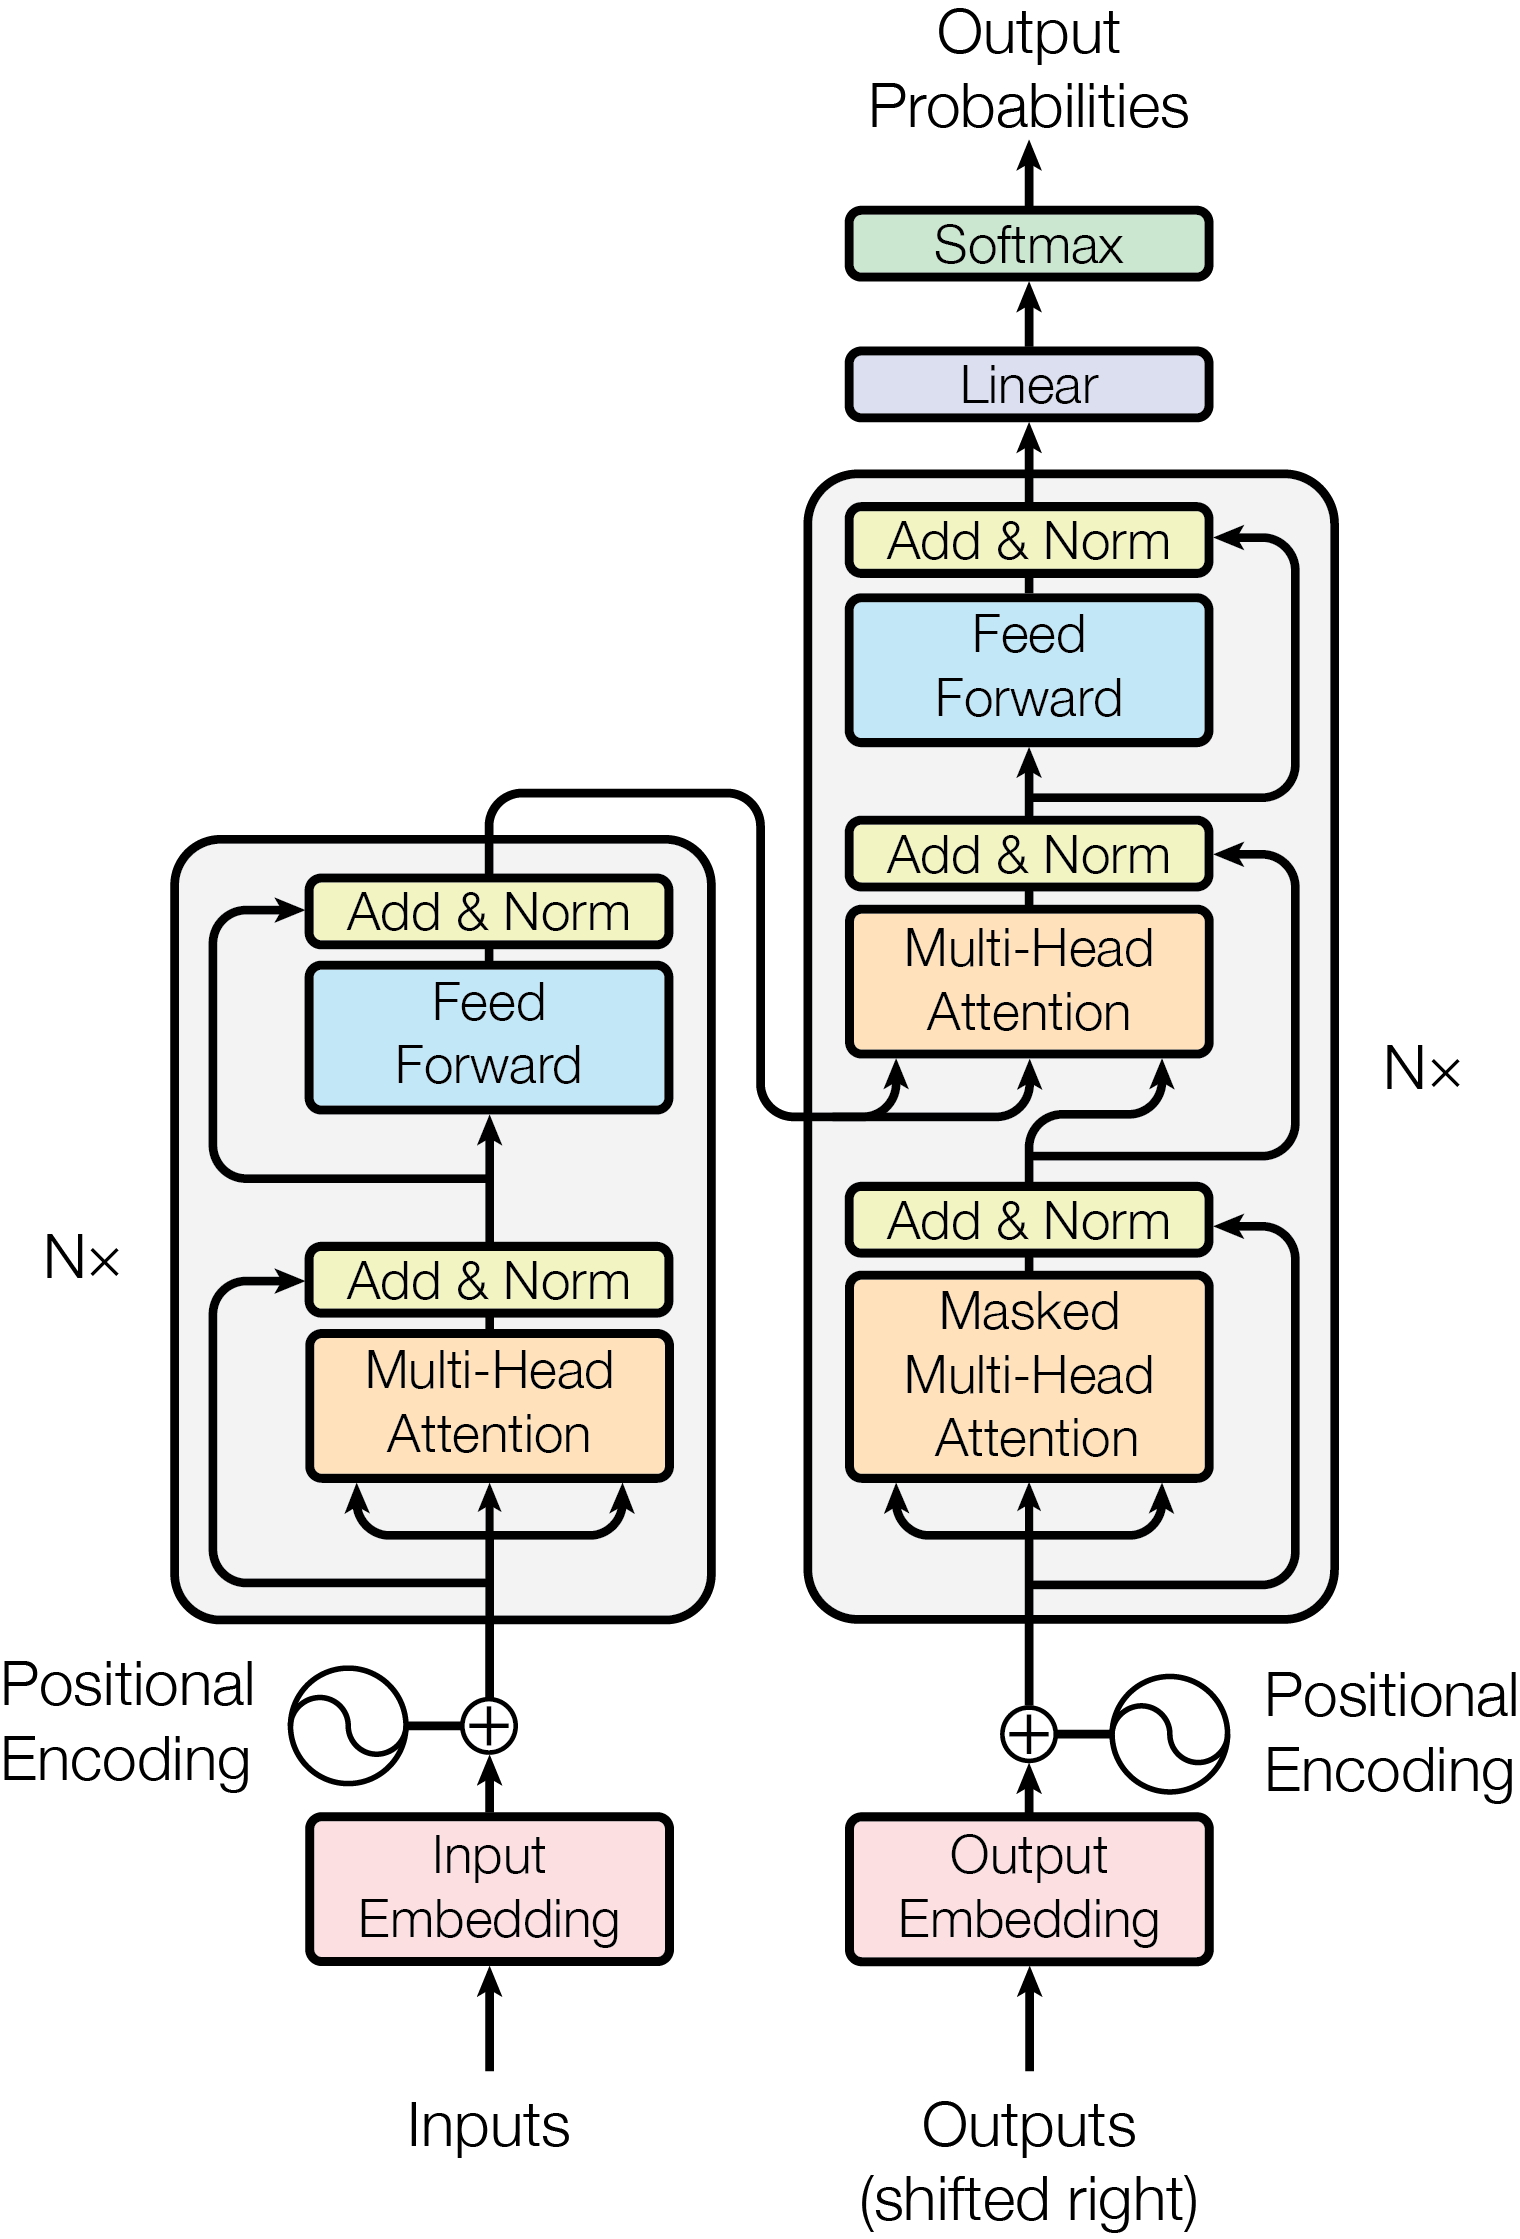
\includegraphics[width=0.4\textwidth]{../10_extra/transformer.png}
   \caption[Transformer Architecture.]{Transformer Architecture \cite{vaswani_attention_2017}.} 
   \label{fig:transformer-architecture}
\end{figure}

\object{Preprocessing Steps} To prepare the text for the transformer model, several steps are performed before the actual encoding and decoding process begins:

\begin{itemize}
   \item \textbf{Tokenization}. It is a crucial step for transformers and \acp{llm}, where the text is parsed into several units called tokens \cite{naveed_comprehensive_2024,raiaan_review_2024,zhao_survey_2025,naik_large_2024}, which represent characters, a group of these or words. With tokens, the next step can be performed.
   \item \textbf{Creating Embeddings}. Each token is then converted into a numeric vector representation of the same dimension \cite{vaswani_attention_2017}. By this, the token's meaning is mapped in a mathematical space, where comparable phrases are close together \cite{raiaan_review_2024}. 
   \item \textbf{Positional Encoding}. As stated in \cite{vaswani_attention_2017}, positional encoding is added to the input embeddings to provide information about the position of each token in the sequence. This is necessary because transformers do not have a built-in order, unlike \acp{rnn} or \acp{cnn}. 
\end{itemize}

\object{Left: Encoder} The encoder structure is primarily designed for processing and interpreting the input text \cite{wang_history_2024}. It extracts step-by-step features and the result is passed to the decoder \cite{liu_understanding_2025}. Each encoder layer consists of two sub-layers: 

\begin{itemize}
    \item \textbf{Orange: Multi-Head Self-Attention} \cite{vaswani_attention_2017}. In this layer, every position in the encoder's sequence can attend to all other positions in the previous layer of the encoder, which is the input of the current layer. By this \cite{liu_understanding_2025}, the model can capture dependencies between differently positioned tokens in the input sequence. 
    \item \textbf{Blue: Position-wise \ac{ffn}} \cite{vaswani_attention_2017}. This layer is applied independently to each position in the sequence. By using this layer \cite{liu_understanding_2025}, the encoder can process and extract features from the attention's output.
\end{itemize}

\object{Right: Decoder} The decoder instead is responsible for generating the output sequence based on the encoded input. This results in a sequence of generated tokens \cite{raiaan_review_2024}. Each decoder layer is a bit different from the encoder layer structure. It consists of the following three sub-layers:

\begin{itemize}
    \item \textbf{Orange$_1$: Masked Multi-Head Self-Attention} \cite{vaswani_attention_2017}. This layer is a modified version of the encoder's self-attention mechanism, but it prevents attending to future sequence positions. By this, the model can only use information from the past tokens and the current one in its decoder layer.
    \item \textbf{Orange$_2$: Multi-Head Attention} \cite{vaswani_attention_2017}. This layer explicitly allows the decoder to attend over the encoder's output, enabling it to incorporate information from the input sequence.
    \item \textbf{Blue: Position-wise \ac{ffn}} \cite{vaswani_attention_2017}. This layer is similar to the one in the encoder, applied independently to each position in the sequence. In the end, the decoder output is passed to a linear layer and a softmax function to finally generate the next-token probabilities.
\end{itemize}

\pagebreak

\object{Resulting Architectures} According to the survey \cite{shao_survey_2024}, the transformer architecture has been split into three main categories, as follows:

\begin{itemize}
   \item \textbf{Encoder-only:} Earlier architectures such as Google BERT \cite{devlin_bert_2019} and its derivates, e.g.\ Huawei ERNIE \cite{zhang_ernie_2019} and Meta RoBERTa \cite{liu_roberta_2019} are solely based on the encoder component. This results a niche for these models being suitable for specific \ac{nlp} tasks focused on comprehension. According to the survey \cite{hou_large_2024}, these models process and encode input into hidden representations to capture word relationships and contextual information. Here, models like BERT observe both the left and right context of the currently focused word.
   
   \item \textbf{Decoder-only}:
   More current models e.g.\ Meta's LLaMA series \cite{touvron_llama_2023}, OpenAI's ChatGPT \cite{openai_introducing_2022} and the publication of GPT-4 \cite{openai_gpt-4_2024} focus on token generation based solely on the preceding tokens \cite{shao_survey_2024}. According to \cite{hou_large_2024}, without the reliance on the encoder, decoder-only transformers can be used for diverse generation tasks, such as code generation and code completion.
   % radford_improving_2018 was deleted GPT-1

   \item \textbf{Encoder-Decoder}: Certain architectures such as Google's T5 \cite{raffel_exploring_2023} and their BART model \cite{lewis_bart_2019} integrate both the encoder and decoder components. This leads to hybrid capabilities, combining the understanding of the input and the proper generation of the output. According to \cite{wang_history_2024}, these models are applicable to e.g.\ machine translation, text summarization and question answering. However, the complexity of the dual architecture can lead to demanding training processes and slower inference times.
\end{itemize}

\object{\ac{moe}} Another notable variant of the transformer architecture is the \ac{moe} \cite{shazeer_outrageously_2017} architecture, as shown in the overview by \cite{naveed_comprehensive_2024}. In this architecture, multiple experts are integrated. Typically, an \ac{moe} system is a mixture of an \ac{ffn} for each expert, positioned right after the attention block, and a router mechanism, which decides which token(s) are processed by which expert(s). These are advantageous in terms of computational efficiency while being as powerful as dense models. That means, the size of the model can be increased without increasing the computational cost proportionally, because only a subset of the experts is activated for each input. % [91,92]
Prominent examples of \ac{moe} models are xAI Grok-1 \cite{xai_open_2024}, Gemini 1.5 by Google \cite{team_gemini_2024-1}, the DeepSeek models V3 \cite{deepseek-ai_deepseek-v3_2025} and its \textit{reasoning} variant R1 \cite{deepseek-ai_deepseek-r1_2025}, and the recently released LLaMA 4 family by Meta \cite{meta_ai_llama_2025}.

\vspace{8em}\pagebreak

\subsection{Framing Bloom's Taxonomy for LLM Applications} \label{sec:blooms-taxonomy}

Given \acp{llm}' capabilities, these enable the automation of the often time-consuming question generation process for educators \cite{vu_chatgpt-based_2024}. The integration of such models into education offers an opportunity to enhance the learning experience for students and support teachers in advancing educational content \cite{naveed_comprehensive_2024}. 
With the help of \acp{llm}, customized study materials and practice questions can be generated to develop personalized learning for students \cite{al_faraby_analysis_2024,bhowmick_automating_2023,hang_mcqgen_2024}, while freeing up the educators' valuable time for both teaching and student interaction \cite{naveed_comprehensive_2024}.
% sources: 452 part 1 / 453.454 for part 2 

\object{Challenge of Alignment} For automated content creation and personalized learning, the ability to differentiate questions based on certain levels of cognitive complexity is crucial \cite{li_planning_2024,zhuge_twinstar_2025}. However, aligning the automated questions with specific cognitive levels still remains a key challenge. \acp{llm} per se show great potential in \ac{aqg} with respect to different cognitive levels \cite{maity_can_2025,blobstein_angel_2023,duong-trung_bloomllm_2024,scaria_automated_2024,scaria_how_2024}. 
By using different prompting strategies, as illustrated in the \bfhyperref{sec:performance-enhancements}{Performance Enhancements} and the according \bfhyperref{sec:question-generation-research}{Question Generation Research} section, the models can be guided to generate questions that are of high quality and better aligned with the cognitive levels of Bloom's Taxonomy. 

Overall, certain approaches can generate questions across all levels by fine-tuning a base model \cite{duong-trung_bloomllm_2024,zhuge_twinstar_2025}, but \cite{duong-trung_bloomllm_2024} lacks the proper evaluation of the cognitive adherence to Bloom's Taxonomy, as the authors' student-based study only evaluated the preference of the generated questions between GPT-4 and their BloomLLM. On the contrary, the authors of TwinStar \cite{zhuge_twinstar_2025} did a thorough but solely automated evaluation of their \ac{aqg} system. In this case, their LLaMA2-based system was compared to \acp{llm} such as GPT-4, and TwinStar outperformed the other models regarding the cognitive adherence. This insight is interesting since the larger models performed worse than the 13 billion parameter version of LLAMA2. Additionally, outdated models were used here and fundamentally in the literature, so the usage of current \acp{llm} can lead to other results. 

However, despite their proficiency at lower levels, \acp{llm} such as ChatGPT \cite{openai_introducing_2022} occasionally struggle with adherence at the higher levels \cite{duong-trung_bloomllm_2024,elkins_how_2023}.
This limitation primarily stems from their tendency to generate questions which are oversimplified or even unrealistic \cite{duong-trung_bloomllm_2024}, or the given cognitive level from the prompt was not properly covered \cite{scaria_automated_2024}. In the latter paper, the evaluation has shown that several \acp{llm} struggle with the adherence to the given cognitive level, but GPT-3.5 and GPT-4 outperformed the other models, such as LLaMA2 \cite{touvron_llama_2023}, by $\approx 20\%$, depending on the prompt specification. In addition to that, generating \textit{Creating}-level questions was the most challenging task for almost every model used in the study. 

Furthermore, in the study of \cite{maity_can_2025}, it was observed that a generated question was better suited to the \textit{Analyzing} level, instead of the \textit{Applying}. It is possible to minimize this problem by prompting the model in a specific way, as the authors have shown via their eight-shot prompting setting. This method requires example context and questions to be provided in the prompt, which is not feasible for every author, as it requires a lot of effort to create the contexts and questions.

\pagebreak

\object{Cognitive Hierarchy} In the literature, as depicted above, Bloom's Taxonomy \cite{krathwohl_taxonomy_1964} and primarily its revised version \cite{krathwohl_revision_2002} are often discussed in the context of question generation and evaluation with respect to \acp{llm} \cite{scaria_automated_2024,scaria_how_2024,elkins_how_2023}.
For crucial understanding of the taxonomy, it follows a hierarchical structure where the six main categories are organized by increasing complexity, with each level building upon a less complex predecessor excepting the lowest level \cite{krathwohl_revision_2002}. The following figure\footnote{\url{https://citt.ufl.edu/resources/the-learning-process/designing-the-learning-experience/blooms-taxonomy/blooms-taxonomy-graphic-description/}, accessed 04/29/2025} shows the cognitive levels of Bloom's Taxonomy in its revised version.

\begin{figure}[htbp]
   \vspace{-.5em}
   \centering
   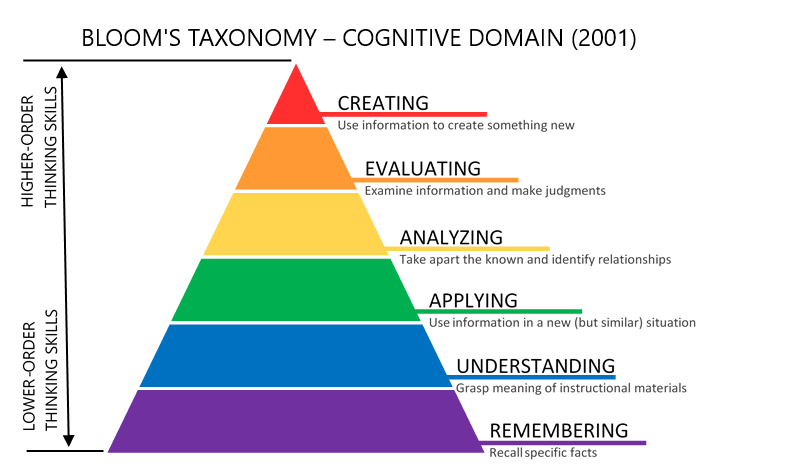
\includegraphics[width=0.65\textwidth]{../10_extra/Blooms-Taxonomy.png}
   \caption{Hierarchy of Bloom's Revised Taxonomy.}
\end{figure}

The revised taxonomy \cite{krathwohl_revision_2002} is divided into six levels. Each level is associated with a specific cognitive skill, as follows with ascending complexity:

\begin{itemize}
   \item \textbf{Remembering:} Formerly known as \enquote{Knowledge}, this level refers to the retrieval of relevant knowledge from long-term memory by focusing on recognition and recall of facts.
   \item \textbf{Understanding:} This level, previously called \enquote{Comprehension}, involves identifying the meaning of instructional messages, such as oral, written and graphic communication.
   \item \textbf{Applying:} This level is about carrying out or using a procedure in a given situation.
   \item \textbf{Analyzing:} This involves breaking down material into its components and determining their relationships to one another or to an overall structure or purpose.
   \item \textbf{Evaluating:} This level requires making judgements based on established criteria and standards.
   \item \textbf{Creating:} This is the highest cognitive level and involves assembling or reorganizing elements into a coherent whole.
\end{itemize}

Each of these cognitive levels is associated with a set of action verbs that can be used to formulate learning objectives and assessment questions. A comprehensive list of such verbs, categorized by these cognitive levels, can be found at the University of Arkansas' website\footnote{\url{https://tips.uark.edu/blooms-taxonomy-verb-chart/}, accessed 05/13/2025}. The following table offers a brief overview of the cognitive levels and their corresponding action verbs:

\pagebreak

\begin{table}[htbp]
   \centering
   \renewcommand{\arraystretch}{1.6}
   \caption{Bloom's Taxonomy Action Verbs.}
   \label{tab:blooms_verbs_columns}
   \begin{tabularx}{\textwidth}{|>{\hsize=1.15\hsize\centering\arraybackslash}X|>{\hsize=1.25\hsize\centering\arraybackslash}X|>{\hsize=0.95\hsize\centering\arraybackslash}X|>{\hsize=0.95\hsize\centering\arraybackslash}X|>{\hsize=0.9\hsize\centering\arraybackslash}X|>{\hsize=0.8\hsize\centering\arraybackslash}X|}
     \hline
     \rowcolor{gray!15}
     \textbf{Remembering} & \textbf{Understanding} & \textbf{Applying} & \textbf{Analyzing} & \textbf{Evaluating} & \textbf{Creating} \\
     \hline
     Define & Clarify & Apply & Analyze & Assess & Assemble \\
     \hline
     Describe & Classify & Calculate & Break down & Conclude & Code \\
     \hline
     Enumerate & Compare & Demonstrate & Detect & Criticize & Compile \\
     \hline
     Identify & Contrast & Determine & Differentiate & Defend & Construct \\
     \hline
     List & Detail & Examine & Distinguish & Evaluate & Create \\
     \hline
     Match & Explain & Illustrate & Examine & Grade & Design \\
     \hline
     Name & Paraphrase & Modify & Investigate & Interpret & Develop \\
     \hline
     Outline & Rewrite & Simulate & Optimize & Judge & Enhance \\
     \hline
     Quote & Summarize & Solve & Relate & Justify & Improve \\
     \hline
     Select & Translate & Use & Separate & Verify & Reorganize \\
     \hline
   \end{tabularx}
 \end{table}

\subsection{Performance Enhancements}
\label{sec:performance-enhancements}

To address these challenges and to refine the capabilities of \acp{llm} for specific tasks, such as \ac{aqg}, various performance enhancement strategies have been proposed. These techniques aim to improve the quality and relevance of the generated content, as listed in the following:

\object{In-Context Learning} As highlighted by \cite{zhao_survey_2025}, the advent of GPT-3 \cite{brown_language_2020} introduced the concept of in-context learning. This method allows \acp{llm} to adapt to new tasks by using a small set of examples directly within the prompt at inference time \cite{minaee_large_2025}. OpenAI further delineated this into subcategories such as zero-shot, one-shot, and few-shot learning, depending on how many examples are provided in the prompt \cite{brown_language_2020}. By this, in-context learning is efficient as it requires minimal task-specific data and no parameter updates in the model itself, while \acp{llm} can adapt without any costly retraining \cite{patil_review_2024,hou_large_2024}.

\object{\ac{cot}} This technique, introduced by Google \cite{wei_chain--thought_2022}, enhances in-context learning by prompting reasoning steps to elicit the \acp{llm}' step-by-step reasoning \cite{zhao_survey_2025}. Moreover, this method can lead to higher quality questions \cite{scaria_automated_2024}, as depicted in \cite{wei_chain--thought_2022}. What makes \ac{cot} so powerful nowadays is that most of the state-of-the-art \acp{llm} are performing techniques like this on their own before returning the final answer to the user \cite{openai_openai_2024-1}, visible in Table \bfref{tab:llm_releases} as the term of \textit{reasoning}.

\object{Role-based Prompting} This technique involves assigning a specific role or persona to the model while prompting it \cite{zhao_survey_2025} to better fulfill the task instruction. The initial phrase of a prompt can look like \enquote{Behave as an expert in the field of $X$}. Independently of the survey \cite{zhao_survey_2025}, the authors of this method \cite{kong_better_2024} have shown that this approach highlights the potential to trigger \ac{cot} implicitly and effectively, leading to enhanced reasoning outcomes. It is worth noting that reasoning here refers to the model's abilities, not the generative step before providing the final answer to the user.

\object{Self-Refinement} By iteratively refining \ac{llm}-generated output based on feedback \cite{madaan_self-refine_2023}, the overall process and the corresponding solutions can be improved \cite{zhao_survey_2025}. For instance, the authors of MCQGen \cite{hang_mcqgen_2024} applied this technique to their \ac{aqg} system, as the model is critiquing and improving its initial outputs in a recursive loop.

\object{Using Special Marks} Emphasizing important parts of the prompt can be achieved by using special marks like quotation marks or line breaks \cite{zhao_survey_2025} to help the \ac{llm} visually distinguish between different parts of the prompt. As an example, to emphasize a text block, it can be enclosed in docstring quotation marks, as it is known from Python programming\footnote{\url{https://peps.python.org/pep-0257/}, accessed 06/16/2025}.

% \object{Positive Constraints} When formulating the prompt, it is often useful to tell the model more what it should do, rather than what it should not do \cite{zhao_survey_2025}, resulting in a balanced and more focused prompt. 

\object{Providing Scoring Standards} For tasks which involve scoring a text, it is crucial to provide a detailed description of the scoring standards in the prompt \cite{zhao_survey_2025}. For instance, using a clear rubric helps the \ac{llm} to assess the quality of generated questions, as it was done in \cite{scaria_automated_2024}. However, in this work -- probably because of the usage of an outdated \ac{llm} --, the evaluation results differ from the human evaluation, which has to be considered when using this technique.

\object{\ac{rag}} This method \cite{lewis_retrieval-augmented_2020}, as used in approach \cite{hang_mcqgen_2024}, highlights how external knowledge sources can be integrated at \ac{aqg} prompts. For this technique, querying a comprehensive database is needed to retrieve relevant information that is useful the context of the question. This can also be realized via e.g.\ knowledge graphs with domain-specific knowledge, which can be based on course content \cite{yang_heuristic_2024}.

\object{Model Fine-Tuning} A key strategy to adapt general-purpose \acp{llm} to specific tasks by training them on domain-specific data \cite{hou_large_2024}. By this process, models can learn knowledge relevant to a specific context, but traditional full fine-tuning requires vast amounts of data and computational resources \cite{hou_large_2024}. For instance, \cite{duong-trung_bloomllm_2024} fine-tuned their \ac{aqg} model BloomLLM with more than 1000 questions, which is still a relatively small amount of data. In the end, this GPT-3.5-based model was preferred across all Bloom levels over GPT-4 according to \ac{aqg}.

\object{Integration of Contextual Knowledge} Several studies \cite{biancini_multiple-choice_2024,blobstein_angel_2023,bhowmick_automating_2023} have injected topic-related contextual information directly into the prompt to avoid hallucinating and give users control over the source of knowledge \cite{biancini_multiple-choice_2024}. 
% #TODO biancini explicitly also assessed the compliance to the source text via experts! 
% # removed wang_towards_2022 from several studies

\pagebreak

\subsection{Evaluation Methodologies}

Evaluation is always necessary to assess the quality of \acp{llm} for the task at hand. According to \cite{doughty_comparative_2024}, evaluating automatically generated learning resources is important because they often lack the deep qualities necessary for their effectiveness.
The methods to evaluate \acp{llm} at e.g.\ \ac{aqg} can be divided into several categories:

\object{$\mathbf{n}$-gram-based Metrics} These metrics follow a reference-based approach, where the generated text is compared to a reference text. The evaluation is based on the overlap of sequences of $n$ words between the generated and reference text \cite{guo_survey_2024}. The most common metrics in this category are:
\begin{itemize}
   \item \textit{\ac{bleu}} \cite{papineni_bleu_2001} evaluates the average $n$-gram precision against a reference text, so how many $n$-grams from the generated text are also present in the reference text \cite{guo_survey_2024}.
   \item \textit{\ac{rouge}}, proposed by \cite{lin_rouge_2004}, calculates recall, which is the ratio of $n$-grams from a ground truth text that are also present in the generated text \cite{guo_survey_2024}.
   \item \textit{\ac{meteor}} \cite{banerjee_meteor_2005} calculates the harmonic mean of precision and recall, so it provides a balanced evaluation \cite{guo_survey_2024}.
\end{itemize}

% -------------------------------------------------------------------------

\object{Diversity-based Metric} The more recent \textit{Distinct-}$n$ \cite{li_diversity-promoting_2016} measures text diversity by calculating the proportion of unique $n$-grams, though it is considered overly simplistic \cite{guo_survey_2024}.

% -------------------------------------------------------------------------

\object{Semantic Similarity} Metrics in this category assess sentence-level comparison, which is vital beyond word-level comparisons \cite{guo_survey_2024}. Regarding \textit{BERTScore} \cite{zhang_bertscore_2020}, it compares contextual sentence-level embedding vectors returned from a pre-trained BERT model. These generated vectors are compared by calculating cosine similarity between the embeddings of the generated and the reference text \cite{guo_survey_2024}, as this scoring metric was adopted in the study of \cite{li_planning_2024}.

\object{Other Metrics} Apart from these categories, diverse other methods and metrics can be used to evaluate the generated questions. For instance, \cite{yang_heuristic_2024} utilized -- besides \textit{Diversity} -- the metrics \textit{Perplexity}, and \textit{Toxicity} to assess the linguistic question's quality. 

In addition to that, researchers developing new evaluation metrics compare their approaches against a range of existing ones. For instance, \cite{nguyen_reference-based_2024} benchmarked their proposed metric against modern metrics e.g.\ \textit{BERTScore}, Google's \textit{\ac{bleurt}} -- predicting human judgements of text quality -- \cite{sellam_bleurt_2020}, and \textit{\ac{rquge}} metric by Meta -- comparing predicted and gold answer spans -- \cite{mohammadshahi_rquge_2023}.

\pagebreak

\object{Human Evaluation} This kind of evaluation is considered necessary to judge about the quality of generated questions \cite{horbach_linguistic_2020}.

\begin{itemize}
   \item While criticizing former used metrics such as \textit{BLEU} and \textit{METEOR} not covering a proper evaluation on question quality, \cite{horbach_linguistic_2020} presented a novel hierarchical evaluation scheme for question generation to guide the human annotators. The scheme often considers binary choices, to induce clear decisions. The following 9 criteria were presented: \textit{Understandable, DomainRelated, Grammatical, Clear, Rephrase, Answerable, InformationNeeded, Central, WouldYouUseIt}. 
   \item Studies such as \cite{steuer_i_2021} and \cite{moore_assessing_2022} adopted this hierarchical scheme and used it for their human question evaluation. For instance, \cite{steuer_i_2021} used it to evaluate their \ac{aqg} system, while \cite{moore_assessing_2022} adopted this scheme to assess the quality of student-generated questions.
   \item Furthermore, the authors of the papers \cite{scaria_how_2024,scaria_automated_2024} used and adapted the evaluation scheme by replacing the criterion \textit{Rephrase} with \textit{Bloom'sLevel}.
   \item Using \cite{moore_assessing_2022} as a reference, \cite{mi_comparative_2024} proposed another scheme with a maximum of 50 points by covering \textit{Relevance, Clarity, Answerability, Challenging} and \textit{Cognitive Level} as criteria. The latter shall present a higher score for student-generated questions that are more cognitively demanding, so these are positioned higher in the Bloom's Taxonomy hierarchy. Focusing on rating student-generated questions, GPT-4 had most voting agreement with expert ratings in contrast to e.g.\ GPT-3.5 and ERNIE.
   % tarrant_frequency_2006 and moore_automatic_2024 removed
\end{itemize}

% -------------------------------------------------------------------------

\object{LLM as an evaluator} Another approach involves using \acp{llm} themselves as evaluators. For instance, \cite{nguyen_reference-based_2024} introduced NACo, an \ac{llm}-based metric that employs a \ac{cot} strategy to rank the \textit{Naturalness, Complexity} and \textit{Answerability} of generated questions. In contrast to this, \cite{scaria_how_2024} employed Gemini Pro\footnote{\url{https://blog.google/technology/ai/google-gemini-ai/\#performance}, accessed 05/09/2025} to assess \textit{Question Quality} and \textit{Alignment} with Bloom's Taxonomy, revealing discrepancies compared to human evaluators. It is noteworthy that the abilities of \acp{llm} are rapidly evolving, and results from former models, e.g.\ Gemini Pro, might differ with versions nowadays. 

% Other research has also explored using \acp{llm} for tasks like classifying question quality, evaluating answerability, or performing other evaluations based on predefined criteria \cite{moore_assessing_2022,scaria_how_2024,blobstein_angel_2023}. 

The use of \acp{llm} for the evaluation of questions is a promising direction, especially when coupled with human evaluation. It is also worth noting that analyzing the inter-rater agreement between the \ac{llm} and the human experts can enhance the reliability of the evaluation process, as it was demonstrated in studies such as \cite{mi_comparative_2024}.

\vp

\section{Related Work} \label{sec:related-work}

This section explores current research in \ac{llms} and their application to \ac{aqg}, with sections to detail the literature review process and highlight significant contributions in the field.

% \newtodo{Discuss other work in the field aiming this related research problem.}
% \newtodo{Show how my research builds on them, where used for inspiration, and e.g. how approaches may be combined.}
% \newtodo{Mention papers, explain why good or bad, also in comparison with my approach.}
% \newtodo{Try to categorize and group the related work by these, show (dis)advantages using one example.}

\object{Literature Review} To find the fundamental principles and state-of-the-art of the research problem, a literature review was conducted. It was performed in the following way: First, several searches were done with respect to \ac{llms} in common, question generation, particularily focusing on Bloom's Taxonomy, and lastly evaluation methods for both categories. Google Scholar and Elicit were used to find relevant papers. Several search terms were coupled in Google Scholar, such as \textit{LLM, Large Language Model, architecture, question generation, automatic question generation, Bloom's Taxonomy, evaluation, assessment, alignment}. Elicit is a search engine that is designed to help researchers find relevant papers based on writing a specific prompt, instead of a query of keywords.

\object{Review Steps} The review steps were as follows: 
\begin{itemize}
    \item First, the papers were downloaded and stored in Zotero. Then, duplicates were filtered out.
    \item The remaining papers were \textbf{included} or excluded by using the TACID method. Papers were included if they are recent (published from 2021 on) and dealing with \ac{llms} or automated question generation or evaluation methods. If the paper was a preprint instead of a peer-reviewed paper, it needed a comparatively high relevance to be included ($\approx 10$ citations). If a publication was present in a workshop, it needed citations to be included.
    \item Papers were \textbf{excluded} if they were not written in English, not open access, or the journal is predatory\footnote{Journals noted on \url{https://beallslist.net/}, accessed 04/30/2025}. If the focus is explicitly on \ac{slms} or multimodal models, or other domains besides the desired ones, the paper was excluded. 
    \item After the process, the remaining papers were filtered by a deeper analysis of the papers.
    \item In the end, diverse cited and subsequently found papers blog posts by e.g.\ Google were added to the thesis to improve the information space.
\end{itemize}

\subsection{Current LLMs Research}

\hspace{1.5em}\object{Review Challenges at \ac{llms}} Finding the current state-of-the-art of \ac{llms} with the explained review method did not yield recent results, even if papers such as surveys were published in 2024 or 2025. The reason for this is that the field of \ac{llms} is moving so fast, that the review papers become outdated. Moreover, the trend of the models and their releases were followed manually, as captured in Table \bfref{tab:llm_releases} below. It shows the most important releases of \ac{llms} in the past years since ChatGPT \cite{openai_introducing_2022}. The table is not complete, but it shows well-known models and their architecture, including \textit{reasoning} capabilities, if these are known to the public. \textit{Reasoning} means, in the OpenAI o1 system card \cite{openai_openai_2024-1} for instance, the model thinks in a manner of \ac{cot} before returning the desired response to the user. The proposed table is sorted by the release date of the models to obtain a timeline and a way to interpret the development of the models.

\begin{table}[htbp]
    \centering
    \caption{Timeline of Major LLM Releases (2022-2025).}
    \label{tab:llm_releases}
    \renewcommand{\arraystretch}{1.4}
    \definecolor{openaiColor}{HTML}{c6e2ce}   
    \definecolor{metaColor}{HTML}{9deade}     
    \definecolor{googleColor}{HTML}{ebd9a1}   
    \definecolor{anthropicColor}{HTML}{cdd8f2}
    \definecolor{xaiColor}{HTML}{efd4d0} 
    \definecolor{deepseekColor}{HTML}{eed6b3} 
    \definecolor{alibabaColor}{HTML}{cde3b5}
    % https://medialab.github.io/iwanthue/

    \begin{tabularx}{\textwidth}{|>{\bfseries\centering\arraybackslash}p{2.5cm}|>{\centering\arraybackslash}p{2.25cm}|>{\centering\arraybackslash}p{4.5cm}|>{\centering\arraybackslash}p{3cm}|>{\centering\arraybackslash}X|}
        \hline
        \rowcolor{gray!15} \textbf{Date} & \textbf{Developers}                            & \textbf{Model Releases} & \textbf{Architecture} & \textbf{Reasoning} \\
        \hline
        Nov 2022                         & \cellcolor{openaiColor}{\textbf{OpenAI}}       & ChatGPT/GPT-3.5         & Decoder-only?         & -- \\ % https://openai.com/index/chatgpt/
        \hline
        \multirow{2}{*}{Feb 2023}        & \cellcolor{metaColor}{\textbf{Meta}}           & LLaMA 65B               & Transformer           & -- \\ % https://arxiv.org/pdf/2302.13971 paper (not really known architecture)
        \cline{2-5}
                                         & \cellcolor{googleColor}{\textbf{Google}}       & Bard 137B               & Decoder-only          & -- \\ % https://ai.google/advancing-ai/milestones/?section=bard is decoder only cuz powered by lamda 137B https://arxiv.org/pdf/2201.08239
        \hline
        \multirow{2}{*}{Mar 2023}        & \cellcolor{openaiColor}{\textbf{OpenAI}}       & GPT-4                   & Decoder-only?         & -- \\ % https://arxiv.org/pdf/2303.08774
        \cline{2-5}
                                         & \cellcolor{anthropicColor}{\textbf{Anthropic}} & Claude 1                & --                     & -- \\ % https://www.anthropic.com/news/introducing-claude
        \hline
        \multirow{2}{*}{Jul 2023}        & \cellcolor{anthropicColor}{\textbf{Anthropic}} & Claude 2                & --                     & -- \\ % https://www.anthropic.com/news/claude-2
        \cline{2-5}
                                         & \cellcolor{metaColor}{\textbf{Meta}}           & LLaMA 2 70B             & Decoder-only          & -- \\ % https://arxiv.org/pdf/2307.09288 paper
        \hline
        Nov 2023                         & \cellcolor{xaiColor}{\textbf{xAI}}             & Grok-1 314B             & MoE                   & -- \\ % https://x.ai/news/grok & https://x.ai/news/grok-os (here MoE)
        \hline
        Dec 2023                         & \cellcolor{googleColor}{\textbf{Google}}       & Gemini                  & Decoder-only          & -- \\ % https://arxiv.org/pdf/2312.11805
        \hline
        Feb 2024                         & \cellcolor{googleColor}{\textbf{Google}}       & Gemini 1.5              & Decoder MoE           & -- \\ % https://arxiv.org/pdf/2403.05530
        \hline
        Mar 2024                         & \cellcolor{anthropicColor}{\textbf{Anthropic}} & Claude 3                & --                     & -- \\ % https://assets.anthropic.com/m/61e7d27f8c8f5919/original/Claude-3-Model-Card.pdf
        \hline
        % Apr 2024                         & \cellcolor{metaColor}{\textbf{Meta}}           & LLaMA 3 70B             & Decoder-only          & -- \\ % https://ai.meta.com/blog/meta-llama-3/
        % \hline
        May 2024                         & \cellcolor{openaiColor}{\textbf{OpenAI}}       & GPT-4o                  & Decoder-only?         & -- \\ % https://arxiv.org/pdf/2410.21276
        \hline
        Jun 2024                         & \cellcolor{anthropicColor}{\textbf{Anthropic}} & Claude 3.5 Sonnet       & --                     & -- \\ % https://www.anthropic.com/news/claude-3-5-sonnet
        \hline
        % Jul 2024                         & \cellcolor{metaColor}{\textbf{Meta}}           & LLaMA 3.1 405B          & Decoder-only          & -- \\ % https://arxiv.org/pdf/2407.21783 paper (dense decoder transformer instead of MoE, presented in Shazeer et al. 2017)
        % \hline
        Aug 2024                         & \cellcolor{xaiColor}{\textbf{xAI}}             & Grok-2                  & --                     & -- \\ % https://x.ai/news/grok-2
        \hline
        Sep 2024                         & \cellcolor{openaiColor}{\textbf{OpenAI}}       & o1-mini                 & --                     & Yes \\ % https://openai.com/index/openai-o1-mini-advancing-cost-efficient-reasoning/
        \hline
        \multirow{4}{*}{Dec 2024}        & \cellcolor{metaColor}{\textbf{Meta}}           & LLaMA 3.3 70B           & Decoder-only          & -- \\ % https://ai.meta.com/blog/future-of-ai-built-with-llama/ and https://huggingface.co/meta-llama/Llama-3.3-70B-Instruct (decoder-only there)
        \cline{2-5}
                                         & \cellcolor{googleColor}{\textbf{Google}}       & Gemini 2.0              & --                     & -- \\ % https://blog.google/technology/google-deepmind/google-gemini-ai-update-december-2024/
        \cline{2-5}
                                         & \cellcolor{openaiColor}{\textbf{OpenAI}}       & o1/o3-mini              & --                     & Yes \\ % https://arxiv.org/pdf/2412.16720 o1 paper, https://openai.com/index/openai-o3-mini/
        \cline{2-5}
                                         & \cellcolor{deepseekColor}{\textbf{DeepSeek}}   & DeepSeek-V3 658B        & MoE                   & -- \\ % https://arxiv.org/pdf/2412.19437
        \hline
        \multirow{2}{*}{Jan 2025}        & \cellcolor{deepseekColor}{\textbf{DeepSeek}}   & DeepSeek R1 658B        & MoE                   & Yes \\ % https://arxiv.org/pdf/2501.12948
        \cline{2-5}
                                         & \cellcolor{alibabaColor}{\textbf{Alibaba}}     & Qwen 2.5-Max            & MoE                   & -- \\ % https://qwenlm.github.io/blog/qwen2.5-max/
        \hline
        \multirow{3}{*}{Feb 2025}        & \cellcolor{xaiColor}{\textbf{xAI}}             & Grok-3                  & --                     & Yes \\ % https://x.ai/news/grok-3
        \cline{2-5}
                                         & \cellcolor{anthropicColor}{\textbf{Anthropic}} & Claude 3.7 Sonnet       & --                     & Yes \\ % https://www.anthropic.com/news/claude-3-7-sonnet
        \cline{2-5}
                                         & \cellcolor{alibabaColor}{\textbf{Alibaba}}     & QwQ-Max                 & MoE                   & Yes \\ % https://qwenlm.github.io/blog/qwq-max-preview/ (based on Qwen 2.5-Max, so MoE)
        \hline
        Mar 2025                         & \cellcolor{googleColor}{\textbf{Google}}       & Gemini 2.5              & --                     & Yes \\ % https://blog.google/technology/google-deepmind/gemini-model-thinking-updates-march-2025/
        \hline
        \multirow{2}{*}{Apr 2025}        & \cellcolor{metaColor}{\textbf{Meta}}           & LLaMA 4 109B/400B/2T    & MoE                   & -- \\ % https://ai.meta.com/blog/llama-4-multimodal-intelligence/
        \cline{2-5}
                                         & \cellcolor{openaiColor}{\textbf{OpenAI}}       & o3/o4-mini              & --                     & Yes \\ % https://cdn.openai.com/pdf/2221c875-02dc-4789-800b-e7758f3722c1/o3-and-o4-mini-system-card.pdf
        \hline
    \end{tabularx}
\end{table}

\pagebreak

\object{Major LLM Developers and Models}
The release of OpenAI's ChatGPT \cite{openai_introducing_2022} has innovated the research on \ac{llms}. Initially leveraging the GPT-3.5 architecture, OpenAI followed the trend of increasing secrecy with models like GPT-4 \cite{openai_gpt-4_2024} and its succesor GPT-4o \cite{openai_gpt-4o_2024}. While the \enquote{GPT} nomenclature suggests the continuation of the decoder-only architecture up to GPT-3 \cite{brown_language_2020}, many methodological details remain undisclosed. Recent models by OpenAI focused on \textit{reasoning} capabilities, as seen in the o1-mini \cite{openai_openai_2024}, o1 \cite{openai_openai_2024-1}, o3-mini \cite{openai_openai_2025}, and the subsequent o3 and o4-mini \cite{openai_openai_2025-1} releases.

Other major developers contributed to this competetive landscape. Meta started with a modified transformer, called LLaMA \cite{touvron_llama_2023}, and shifted to a decoder-only architecture in LLaMA 2 \cite{touvron_llama_2023-1} up to LLaMA 3.3\footnote{\url{https://github.com/meta-llama/llama-models/blob/main/models/llama3_3/MODEL_CARD.md}, accessed 05/09/2025. Note that auto-regressive means decoder-only}. With the release of the LLaMA 4 family \cite{meta_ai_llama_2025}, Meta switched to the \ac{moe} architecture, scaling its largest model to two trillion model parameters. Google followed a similar path, switching from its LaMDA-based Bard \cite{pichai_important_2023,thoppilan_lamda_2022} to the now well-known Gemini model series \cite{team_gemini_2024} by fine-tuning Bard. The family also started as decoder-only, while Gemini 1.5 marked a shift to an \ac{moe} architecture, though still described as decoder-based \cite{team_gemini_2024-1}. Beginning with Gemini 2.0 \cite{pichai_introducing_2024}, Google stopped publishing detailed architectural information. Gemini 2.5 \cite{kavukcuoglu_gemini_2025} further advanced their offerings by fully integrating reasoning capabilities, aligning with current state-of-the-art trends.

Besides the presented developers, Anthropic has remained private about architectural information of its Claude models, from Version 1 \cite{anthropic_introducing_2023}, Claude 2 \cite{anthropic_claude_2023}, through the Claude 3 family \cite{anthropic_introducing_2024-1}, Claude 3.5 Sonnet \cite{anthropic_introducing_2024} up to Claude 3.7 Sonnet \cite{anthropic_claude_2025}. The latter model also incorporated \textit{reasoning}, making it competitive with other currently leading models. Meanwhile, developers such as xAI, DeepSeek AI, and Alibaba have set up several \ac{moe} models. xAI's Grok-1 was openly an \ac{moe} model \cite{xai_open_2024}. However, for subsequent releases, Grok-2 \cite{xai_grok-2_2024} and Grok-3 \cite{xai_grok_2025}, architectural details were not provided, though Grok-3 is a competitive state-of-the-art model with \textit{reasoning}. DeepSeek AI has contributed powerful open-source \ac{moe} models like DeepSeek V3 \cite{deepseek-ai_deepseek-v3_2025} and its reasoning variant, R1 \cite{deepseek-ai_deepseek-r1_2025}. Similarly, the Alibaba Group has also contributed to the field with models like Qwen 2.5-Max \cite{team_qwen25-max_2025}, an \ac{moe} model. The more recent QwQ-Max \cite{team_thinkthink_2025} builds upon this architecture, incorporating reasoning to compete at the state-of-the-art.

Visible in Table \bfref{tab:llm_releases}, the current state-of-the-art for the given table began from o1 and o3-mini in December 2024 plus the release of DeepSeek V3. January 2025, DeepSeek R1 and Alibaba's Qwen 2.5-Max model without reasoning capability were released. February 2025 brought xAI's Grok-3, Anthropic's Claude 3.7 Sonnet and Alibaba's QwQ-Max. In March 2025, the state-of-the-art was reached by a major upgrade in Google Gemini, with the release of Gemini 2.5. Finally, April 2025 featured the LLaMA 4 family by Meta and OpenAI's o3 and o4-mini models. Based on this information pool, the models for the \ac{aqg} evaluation were selected, as to be seen in Section \bfref{sec:experiment-design}. 

\pagebreak

\object{Key \ac{llm} Development Trends} As illustrated in Table \bfref{tab:llm_releases}, a discernible trend is the decreasing transparency from developers regarding architectural designs of their \ac{llms}. While some models are known to be transformer-based (e.g.\ decoder-only) or employ an \ac{moe} architecture, and reasoning capabilities are often highlighted, many other details remain undisclosed due to the competitive nature of the field. It is also worth noting that there is a trend towards models with a higher number of parameters, a prevalence of decoder-only architectures from ChatGPT on, and an increasing adoption of \ac{moe} designs, a trend possibly popularized by GPT-4. Although the technical report for GPT-4 \cite{openai_gpt-4_2024} lacks architectural specifications, it is rumored to be an \ac{moe} model\footnote{\url{https://medium.com/@seanbetts/peering-inside-gpt-4-understanding-its-mixture-of-experts-moe-architecture-2a42eb8bdcb3}, accessed 05/09/2025}. Furthermore, a significant trend is the continuous integration of reasoning capabilities into \ac{llms}, with the most recent models being competitive in this area.

\subsection{Question Generation Research}
\label{sec:question-generation-research}

\ac{llms} enable the automation of the time-consuming and demanding procedure of question generation \cite{vu_chatgpt-based_2024}. As stated by \cite{naveed_comprehensive_2024}, the integration of \ac{llms} into educational settings offer an opportunity to improve the learning experience, support teachers and encourage the development of educational content. This results in freeing up time for educators to focus on teaching and interacting with students. Two certain directions of research are presented in the following:

\object{Prompt Engineering Approaches} Numerous studies have investigated the capability of \ac{llms} to generate educational questions, primarily aligned with cognitive levels, by solely refining and optimizing the prompts given to the models.

\cite{scaria_how_2024} addressed the problem of creating pedagogically effective questions, especially at higher skill levels, which is challenging, time-consuming, and requires expert-based evaluation. By this, researchers can understand the pedagogical aspects of \ac{aqg}, since automated metrics often analyze linguistic features. The study assessed the capability of \ac{llms}, including GPT-3.5 and GPT-4 and other models, to generate high-quality questions across different cognitive levels by using zero-shot prompting. The question evaluation was conducted by two annotators based on the categories adopted from \cite{horbach_linguistic_2020}, replacing the \textit{Rephrase} category with \textit{Bloom'sLevel}. This category assesses the adherence to the targeted cognitive level. The Inter-annotator agreement was measured using Cohen's Kappa \cite{cohen_coefficient_1960}, since there are two annotators to be validated. Their findings revealed that over $91\%$ of the generated questions were relevant and high-quality, where models such as GPT-4 and GPT-3.5 were notably effective, especially in adhering to the desired Bloom level. However, limitations were identified by the authors, e.g.\ the crucial human evaluation can be subjective. Also, most models were unable to generate high-quality questions at the \textit{Apply} and \textit{Create} levels, and the study lacked prompt diversity, as the same zero-shot prompt was used for all models.

\pagebreak

\cite{maity_can_2025} have described the gap that frameworks like Bloom's Taxonomy are often not fully integrated into the systematic assessment of generated questions, or they have not employed comprehensive methods to determine the completeness and relevance of the questions. Their research explored the potential of \ac{llms} -- such as several GPT and LLaMA models plus Gemini Pro -- for \ac{aqg} by comparing zero-shot prompting against eight-shot prompting. By this, they generated a complete set of questions aligned with Bloom's Taxonomy using school textbooks. Using the same evaluation metrics as \cite{elkins_how_2023}, the teachers-based evaluation indicated that eight-shot prompting improved the quality and Bloom adherence of educational questions. GPT-4 was identified as the best performing model under both prompting conditions. As future work, the authors suggested exploring 16- and 32-shot prompting, which could further enhance the quality of generated questions. However, they have not addressed the subjective nature of human evaluation, because 28 teachers were involved in the evaluation process, which could lead to a more diverse assessment of the generated questions.

The authors of \cite{al_faraby_analysis_2024} also stated that the quality and pedagogical effectiveness of \ac{llm}-generated questions have not been thoroughly evaluated. Furthermore, \ac{llm}-based question generation, which aims to meet educational objectives, is unexplored. The assessment of these questions plus the comparison with expert-generated ones is the focus of their study, primarily using ChatGPT. While disregarding frameworks such as Bloom's Taxonomy, the study focused on textbook-based questions and different prompting strategies: zero-shot, enhanced zero-shot, few-shot, and few-shot with \ac{cot}, where each strategy was tested with 6 variations. Human evaluators -- experts and crowdsourced workers -- were employed to assess the generated questions. The results revealed that experts preferred human-generated questions from textbooks, while the crowdsourced evaluators have shown comparable preferences for both human- and \ac{llm}-generated questions. However, the authors also highlighted the issue of hallucination, which remains a challenge in \ac{aqg}. They suggested that future work should focus on integrating systems to verify questions against source texts. Moreover, the study had a small -- but unknown -- number of annotators. They suggested a broader range of \ac{llms} and a higher variety of questions to be included in future work.

Traditional \ac{aqg} systems struggle to generate questions at higher cognitive levels, and they often lack control over question complexity and difficulty \cite{blobstein_angel_2023}. Prior work has focused on incorporating pre-formulated answers into the question generation process. Addressing this, the authors developed Angel, a tool that utilizes GPT-3.5 for generating questions and answers based on learning material. The system employs instructional prompts for \ac{aqg} and evaluation -- including few-shot prompting, descriptions for the Bloom levels, and textbook content to produce questions categorized by difficulty (easy, medium, hard). On the one hand, the evaluation of the generated questions was conducted using GPT-3.5 again as an evaluator with a \ac{cot} strategy, focusing on metrics such as \textit{Clarity, Relatedness, Importance,} and \textit{Answerability}. On the other hand, human evaluation was also performed, coupled with GPT-3.5 for assessing the resulted Bloom levels of the questions. While the LLM-based evaluation indicated that Angel generated more questions at higher cognitive levels -- in contrast to the contestant systems -- the human evaluation underscored that the majority of the questions were still classified as \textit{Remembering}. The authors concluded that while Angel demonstrated potential for \ac{aqg}, further work and human evaluation are needed to analyze the results more accurately.

\object{Hybrid Architectures} Researchers have also developed more complex systems that integrate \ac{llms} with other components in a coordinated fashion. These hybrid architectures often aim to leverage the strengths of different techniques to achieve more robust and diverse question generation.

In contrast to the previous studies, \cite{doughty_comparative_2024} addressed the gap of generating \ac{mcqs} in programming education, which is linked with much effort. \ac{llms} were not thoroughly explored for this purpose, since evaluating systems which generate \ac{mcqs} is limited. The authors conducted a comparative study of \ac{mcqs} generated by GPT-4 versus those created by humans. In addition to the \ac{llm}, few-shot prompting, course context and learning objectives aligned with Bloom's Taxonomy levels -- realized through fine-tuned BERT classifier -- were used for \ac{aqg}. The resulted questions were comparable to human-generated ones in terms of clarity and learning objective coverage. Nevertheless, limitations included potential bias from human evaluators, the focus on programming questions, and the need to consider the alignment between the question and the learning content, as depicted similarly in \cite{al_faraby_analysis_2024} above.

Focusing on personalized learning, \cite{hang_mcqgen_2024} described that both efficient and effective generation of \ac{mcqs} is essential in modern teaching, since the manual generation is depicted as resource-intensive and time-consuming. Their system, MCQGen, utilizes GPT-4, \ac{rag}, and advanced prompting techniques to automate the creation of personalized \ac{mcqs} while accessing an external knowledge base. The self-refinement and \ac{cot} prompting were employed to enhance the quality of the generated questions. Assessing the questions based on \textit{Grammar, Answerability, Diversity, Complexity,} and \textit{Relevance}, the outcomes between the three \ac{llm}-based evaluators and three lecturers were mixed. In this work, especially the \textit{Complexity} and \textit{Diversity} metrics were lacking in both evaluation methods, suggesting that prompt optimization and expanding the knowledge base could address these limitations. In addition to that, the usage of only one \ac{llm} coupled with the focus on computer science questions in English language were also limitations of this work.

\subsection{Research Gaps Addressed}

Based on the conducted literature review, presented in the previous sections of the thesis, there are several research gaps this work aims to address: 

\object{Outdated Models} Current studies rely on \ac{llms} from 2023 or earlier, such as GPT-4, GPT-3.5, and LLaMA2 \cite{scaria_how_2024, maity_can_2025, al_faraby_analysis_2024}. These evaluations lack in capturing the capabilities of recent models that incorporate advanced \textit{reasoning} mechanisms to think before answering. To address this, the thesis investigates four current state-of-the-art models, as detailed in Section \bfref{sec:experiment-design}. This ensures that the evaluation of \ac{aqg} capabilities is conducted using the most recent technologies, resulting in a more up-to-date understanding of \ac{llms}' potential in educational contexts.

\pagebreak

\object{Limited Content Adherence Evaluation} A persistent challenge in \ac{aqg} is the problem of hallucination, which is unacceptable in education \cite{yang_heuristic_2024}. \ac{llms} can generate misleading or irrelevant information which are not directly supported by e.g.\ the source text \cite{al_faraby_analysis_2024,duong-trung_bloomllm_2024}. While some studies mention this issue, the content adherence between a provided context and the generated questions still remains underexplored, as stated in the limitations of e.g.\ \cite{doughty_comparative_2024,al_faraby_analysis_2024}. This thesis investigates this problem in RQ1 -- conducting both quantitative and qualitative analysis. This kind of evaluation is crucial for generating reliable educational questions that can be answered accurately using the source material, as diverse materials were used in e.g.\ \cite{scaria_how_2024,maity_can_2025,blobstein_angel_2023}. Highlighted in related research \cite{biancini_multiple-choice_2024}, it is important to inject knowledge directly into prompts to contrast hallucinations and give educators control over the source text.

\object{Bloom's Taxonomy Integration and qualitative Evaluation} While several studies have incorporated Bloom's Taxonomy into \ac{aqg} evaluation \cite{scaria_how_2024, maity_can_2025, blobstein_angel_2023}, most research lacks comprehensive analysis of how different question formats perform across various cognitive levels. Existing work primarily focuses on adherence to specified Bloom levels without examining the relationship between question types (e.g.\ Multiple-Choice vs. Open-Ended) and their pedagogical effectiveness at different cognitive complexities. In addition to that, the \ac{llms} used struggle with higher cognitive levels \cite{blobstein_angel_2023}, such as \textit{Apply} and \textit{Create} \cite{scaria_how_2024}. Since these models are far from the state-of-the-art, there is an opportunity to explore how the latest \ac{llms} perform in generating questions at all six Bloom levels, while several publications did not include Bloom's Taxonomy into their work \cite{al_faraby_analysis_2024,vu_chatgpt-based_2024,hang_mcqgen_2024}. 

Furthermore, many studies rely heavily on automated metrics or limited human evaluation \cite{zhuge_twinstar_2025,blobstein_angel_2023,li_planning_2024} -- often with few annotators --, which might not capture the full pedagogical value of generated questions. This thesis addresses this mixed gap primarily through RQ2 by conducting a comprehensive analysis of question format performance across all six Bloom levels, employing expert-based evaluation with established inter-rater agreement measures. The evaluation framework incorporates rubrics that assess not only Bloom level adherence but also qualitative criteria, providing a proper understanding of \ac{llm} capabilities in \ac{aqg}. The rubrics for both experiments are proposed in Section \bfref{sec:experiment-design} and are based on the work \cite{mi_comparative_2024}.

This set of research gaps highlights the need for a comprehensive evaluation that can evaluate modern \ac{llms} in \ac{aqg} using current methods. The proposed framework in the section below aims to bridge the research gaps and provide a foundation for future research in \ac{aqg} and \ac{llms}.
\vp

\section{Experimental Design}
\label{sec:experiment-design}

Two experiments were conducted to evaluate the performance of a selected set of \ac{llms} -- using solely \textit{reasoning} models -- in generating questions. The first experiment primarily focused on the \textbf{RQ1}, which aimed to assess the content fidelity of the generated questions according to the \ac{llms} and the diverse source materials. The second experiment was designed to answer \textbf{RQ2}, which focused on analyzing the relationships between the \ac{llms}, given questions formats and given levels of Bloom's revised Taxonomy \cite{krathwohl_revision_2002}.

\begin{figure}[htbp]
    \centering
    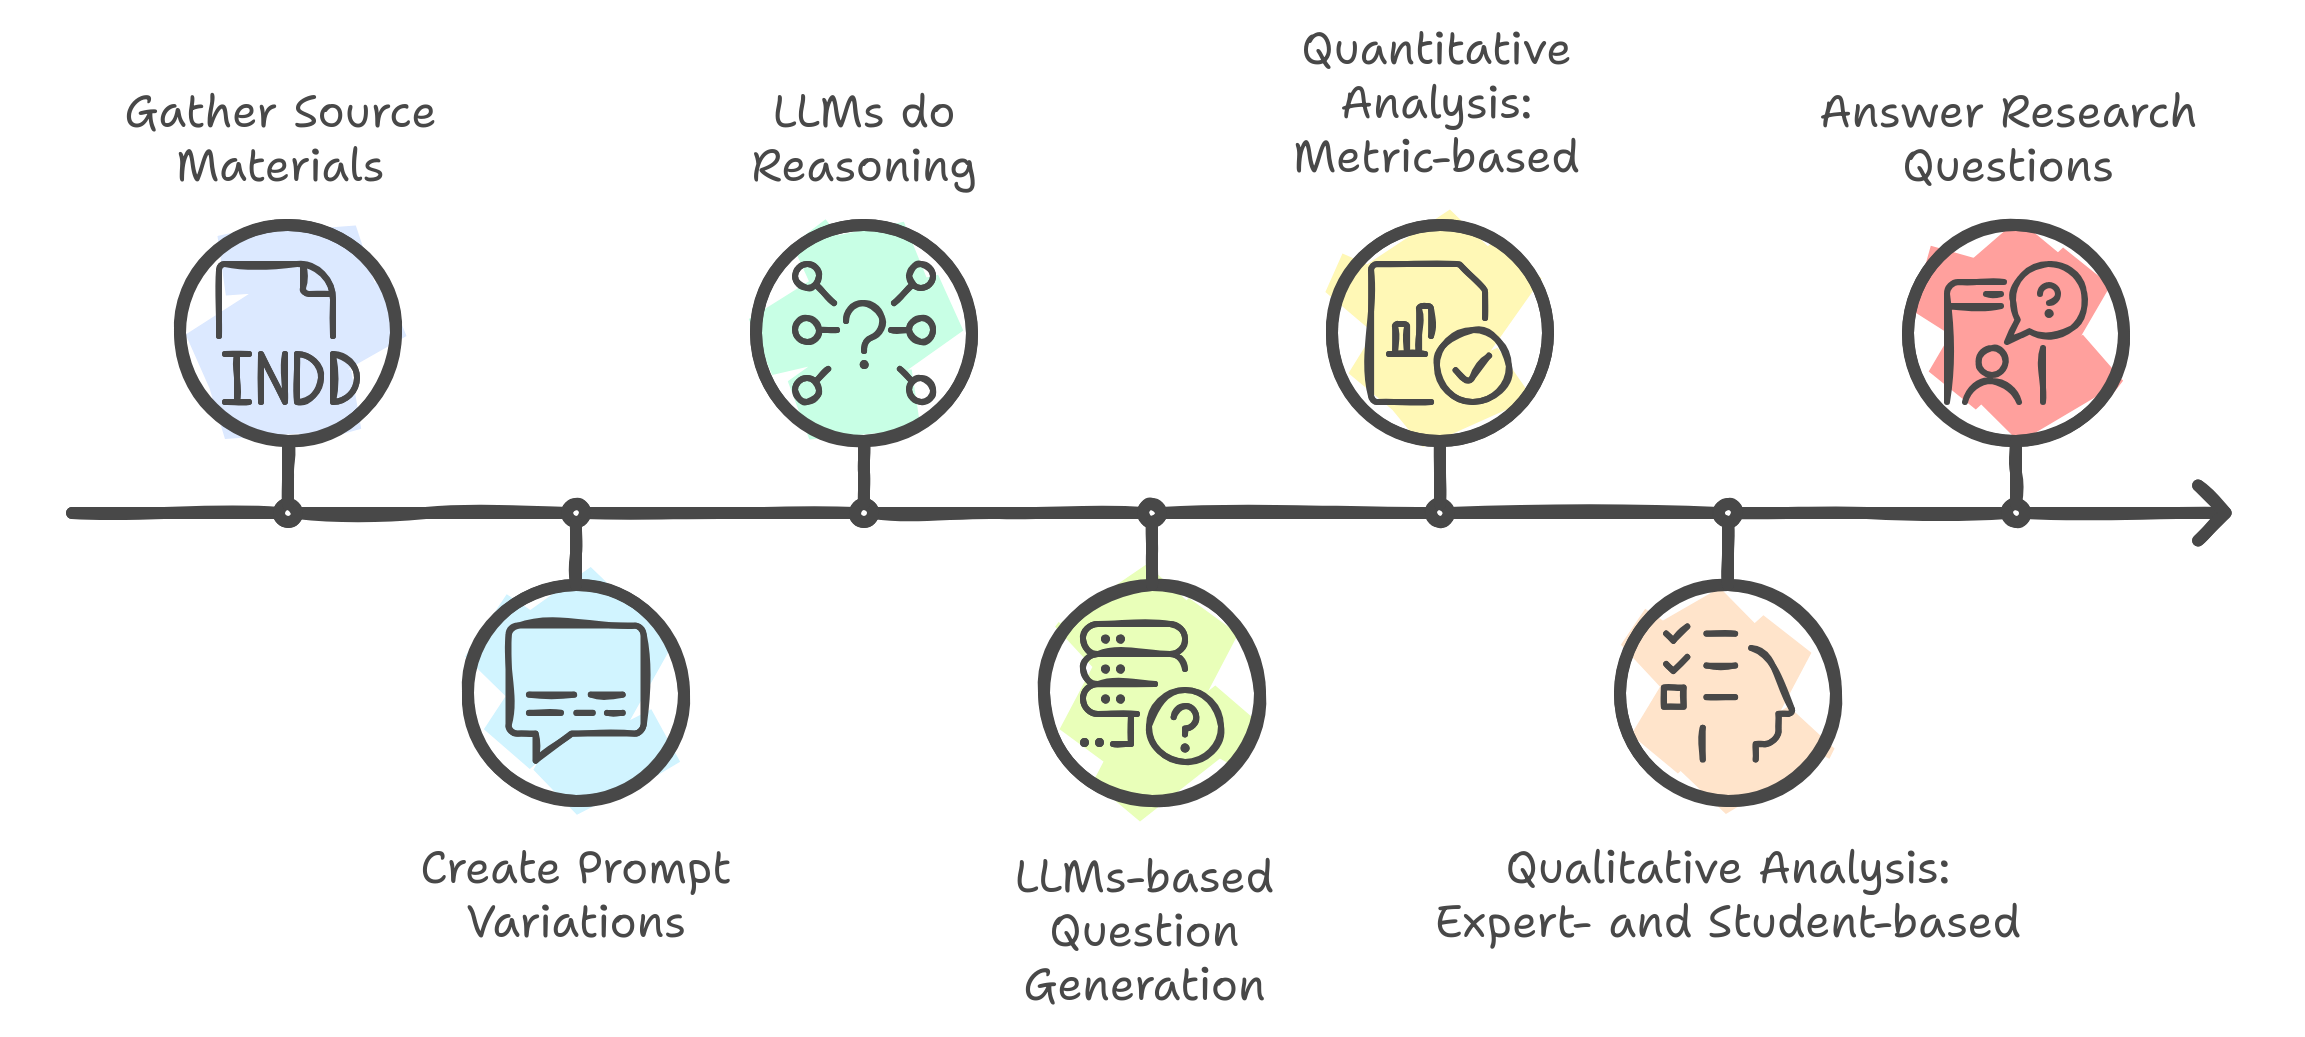
\includegraphics[width=.9\textwidth]{../10_extra/approach.png}
    \caption[Experimental Pipeline.]{Experimental Pipeline\footnotemark.}
    \label{fig:experiment-overview}
\end{figure}
\footnotetext{created with \url{https://www.napkin.ai/}, accessed 05/24/2025}
\vspace{-1em}
    
\subsection{Selection of Resources}
\label{sec:selection-resources}

To ensure the experiments were well-structured and relevant, a variety of resources were selected. This covers the source materials and the \ac{llms} used in the experiments for \ac{aqg}.

\object{Selection of Source Materials}
Focusing on the ISO-OSI model, the following materials, illustrated in its \bfhyperref{sec:source_materials}{Appendices} subsection, were diversely used to generate the experiments' questions:

\begin{itemize}
    \item \bfhyperref{sec:script-common}{Lecture Slides} \textbf{(extracted Parts)}: Dealing with reference architectures, the ISO-OSI model is presented in detail by the primary thesis supervisor. The lecture slides are in German and were used for \ac{aqg} for both experiments.
    \item \bfhyperref{sec:transcript}{Transcript} \textbf{(Lecture's Video Parts)}: The transcript of the extracted slides is in German and was also used to generate questions for the first experiment.
    \item \bfhyperref{sec:tanenbaum}{Book's Excerpt} \textbf{(from \enquote{Computer Networks})} \cite{tanenbaum_computer_2013}: This book is in English and was used to generate questions for both experiments, with a detailed description of the ISO-OSI model, including all seven layers.
\end{itemize}

\pagebreak

To properly challenge the \ac{llms} in their multilingual capabilities, each source material was kept in its original language: German for the lecture slides and its transcript, the book excerpt in English.

% \pagebreak

\object{Selection of \ac{llms}} A total of four \ac{llms} were selected for both experiments, which belong to the current state-of-the-art in the field of \ac{llms} and are publicly available to certain degrees, and incorporate reasoning capabilities. The selected models are:
Anthropic Claude 3.7 Sonnet \cite{anthropic_claude_2025},
    DeepSeek R1 \cite{deepseek-ai_deepseek-r1_2025},
    Google Gemini 2.5 Flash \cite{kavukcuoglu_gemini_2025}, and
    OpenAI o3 \cite{openai_openai_2025-1}.

\vspace{1em}

o3 and Claude 3.7 Sonnet were accessed through their Python APIs\footnote{\label{fn:openai-api}\url{https://github.com/openai/openai-python}, accessed 05/09/2025}\footnote{\label{fn:anthropic-api}\url{https://github.com/anthropics/anthropic-sdk-python}, accessed 05/09/2025}, incurring costs per usage. This access method was necessary as the chosen models were not available to the required extent through other means. In contrast, Gemini 2.5 Flash was utilized via Google's Python API\footnote{\label{fn:google-api}\url{https://github.com/googleapis/python-genai}, accessed 05/09/2025}, which offers a free usage tier. To manage costs while maintaining a robust set of \ac{llms}, DeepSeek R1, a comparatively less expensive yet highly capable \ac{llm}, was accessed free of charge via its website\footnote{\label{fn:deepseek}\url{https://chat.deepseek.com/}, accessed 05/09/2025}.

\subsection{Methodological Approach}
\label{sec:methodological-approach}

The method employed for the two experiments is outlined here. It details the specific procedures for generating questions, including the variations in source materials, \ac{llm} prompting strategies, and the targeted number of questions for each experimental condition.

\object{Experiment 1a: Content Fidelity} For the first experiment, questions were generated using the three selected source materials to compare the questions' quality. All four state-of-the-art \ac{llms} were employed. Each model was prompted using both a simple and a complex prompt. To prevent context spillover and ensure focused questioning, one question was generated per prompt for each of the seven layers of the ISO-OSI model, with the context for each layer being introduced in each distinct run. This methodology resulted in a total of
 \begin{align}4 \text{ \ac{llms}} \times 3 \text{ input sources} \times 7 \text{ layers} \times 1 \sfrac{\text{ question}}{\text{prompt}} \times 2 \text{ prompts} = 168 \text{ questions.}\end{align}

\object{Experiment 1b: Error Handling} A subsequent run focused on error handling. The four \ac{llms} were again utilized with the same prompts. For this experiment, a single input source, specifically the lecture script -- chosen for its concise and precise contextual information -- was used. Each of the seven layers of the ISO-OSI model within this source material was intentionally manipulated to introduce errors, as to be seen in its \bfhyperref{sec:script-manipulated}{Appendices} subsection. Seven questions were generated per prompt, one for each manipulated layer and run. This resulted in a total of \begin{align}4 \text{ \ac{llms}} \times 1 \text{ input source} \times 7 \text{ layers} \times 1 \sfrac{\text{ question}}{\text{prompt}} \times 2 \text{ prompts} = 56 \text{ questions.}\end{align}

\pagebreak

\object{Experiment 2: Question Formats and Bloom's Taxonomy} The second experiment focused on the generation of varied question formats and their alignment with Bloom's revised Taxonomy. Contextual information for this experiment was derived from all ISO-OSI model layers together, utilizing the precise lecture \bfhyperref{sec:script-common}{Script} by the primary thesis supervisor. The four selected \ac{llms} were employed in three distinct runs, each designed to explore different prompting parameters related to question type and cognitive complexity:

\begin{enumerate}
    \item \textit{Question Type Specification}: Prompts specified only the desired question types (Multiple-Choice and Open-Ended). For the chosen layer, each \ac{llm} was tasked six times to generate a question without mentioning a certain Bloom level for each of the two question types, resulting in \begin{align}4 \text{ \ac{llms}} \times 2 \text{ question types} \times 1 \sfrac{\text{ question}}{\text{run}}\times 6 \text{ runs} = 48 \text{ questions.}\end{align}
    \item \textit{Cognitive Level Specification}: Prompts specified only the target cognitive levels according to Bloom's Taxonomy. For the chosen layer, each \ac{llm} generated one question for six runs to get a question for each of the Bloom levels. In total, these are  \begin{align}4 \text{ \ac{llms}} \times 1 \sfrac{\text{ question}}{\text{level}} \times 6 \text{ Bloom levels} = 24 \text{ questions.}\end{align}
    \item \textit{Combined Specification}: Prompts specified both the question types (Multiple-Choice and Open-Ended) and the cognitive levels. Similar to the first run, this resulted in \begin{align}4 \text{ \ac{llms}} \times 2 \text{ question types} \times 1 \sfrac{\text{ question}}{\text{level}} \times 6 \text{ Bloom levels} = 48 \text{ questions.}\end{align}
\end{enumerate}

\object{Data Collection} The data was primarily collected using the \ac{llms} via their APIs, excepting DeepSeek being prompted on the website. The other 3 models were prompted automatically via Python to generate questions based on the given source materials. The generated questions were stored in a directory structure, particularly based on the experiment, the \ac{llm} and the source material. The question files for each prompt were stored in distinct \textit{.txt} files.

\object{Evaluation Plan} The evaluation will be conducted in two phases, one for each experiment. These employ a multi-modal assessment combining automated metrics and expert annotation -- the primary supervisor, staff members, and students -- to ensure a comprehensive quality assessment.

\begin{itemize}
    \item \textbf{Experiment 1 (Content Fidelity and Error Handling):}
    \begin{itemize}
        \item \textit{Quantitative Analysis:} In this stage, the \textit{Semantic Similarity} between each generated question and the desired source material will be evaluated. Instead of relying directly on BERTScore \cite{zhang_bertscore_2020}, the cosine similarity between the embedding vectors -- representing the source material and the generated question -- will be computed. These embeddings are obtained using a cross-lingual RoBERTa-based sentence transformer\footnote{\url{https://huggingface.co/T-Systems-onsite/cross-en-de-roberta-sentence-transformer}, accessed 05/09/2025}, which produces semantically meaningful and comparable sentence representations \cite{reimers_sentence-bert_2019}.
        
        Novel metrics such as \textit{\ac{bleurt}} and \textit{\ac{rquge}} were not employed since, on the one hand, the structure of the source material and the question differ too much, and on the other hand, gold standard answers are not available for comparison.

        Moreover, other metrics such as Perplexity are unsuitable for this task, as \enquote{the output value is based heavily on what the text and the model was trained on. This means that perplexity scores are not comparable between models or datasets}\footnote{\url{https://huggingface.co/spaces/evaluate-metric/perplexity}, accessed 06/01/2025}. Instead, to properly analyze the content adherence on a quantitative level besides the \textit{Semantic Similarity}, the \textit{Adherence Score} will be introduced in this thesis as an alternate quantitative scoring method. It will be assessed by prompting Claude 3.7 Sonnet and OpenAI o3 for every question with its desired source material to obtain acceptable results, using the mean of both \ac{llm} values. This results in a value between 0 and 1 for each question, presenting the adherence to the source material.

        \item \textit{Qualitative Analysis:} This phase involves a blind-test with expert-based evaluations of the generated questions. Five experts, including the primary thesis supervisor and four scientific staff members from the same university department of Information and Communication Services, will rate a sampled question set using the concise rubric in Table \bfref{tab:exp1_criteria}. To analyze the inter-rater agreement between the experts, Fleiss' Kappa will be calculated, which is suitable for analyses carried out by at least two raters \cite{fleiss_measuring_1971}.
        
        The thesis' analysis adopts the rubric from \cite{mi_comparative_2024} -- based on criteria by \cite{moore_assessing_2022} --, which maintains a maximum score of 50 points per question. However, instead of the \textit{Bloom's Level} criterion, the \textit{Correctness}, the \textit{Value} from the lecturer's perspective, and the \textit{Language} criteria were added to address the objectives of this experiment.
        
        Since Experiment 1b examines the adherence to manipulated input texts, the \textit{Correctness} is then replaced by \textit{Manipulation Handling}, respectively. To distinguish between the \textit{Clarity} and \textit{Language} criteria, clarity focuses on content clarity and logical comprehension, while language assesses linguistic complexity and precision of expression.

\begin{table}[htbp]
           \vspace{-5em}
           \centering
           \renewcommand{\arraystretch}{1.8}
           \caption{Experiment 1 Evaluation Criteria.}
           \label{tab:exp1_criteria}
           \begin{tabularx}{\textwidth}{|Z|A|Y|}
           \rowcolor{gray!15}
           \hline
           \textbf{Criterion} & \textbf{Description} & \textbf{Scoring} \\
           \hline
           \textbf{Relevance} & Is the question relevant to the topic of the source text? & 0-10p \\
           \hline
           \textbf{Clarity} & Is the question easy to understand \& the presentation logical and clear? & 0-10p \\
           \hline
           \textbf{Answerability} & Are students likely able to answer the question based on the provided material? & 0-10p \\
           \hline
           \textbf{Challenging} & Is the question challenging? Does it encourage students to think actively? & 0-10p \\
           \hline
           \textbf{Value} & Is the question considered professionally, didactically, or technically meaningful by the instructor? & 0-10p \\
           \hline
           \textbf{Language} & Is the language used by the system sufficiently precise and comprehensible? & 0-10p \\
           \hline
           \textbf{Correctness} & \textbf{For Experiment 1a:} Is the question factually correct \& adhering to the source text? & \vspace{-1.1em}\begin{itemize} 
                \item Correct: 10p
                \item Partially correct: 5p
                \item Otherwise: 0p
            \end{itemize} \\
           \hline
           \textbf{Manipulation Handling} & \textbf{For Experiment 1b:} Does the question adhere to the manipulated input text content? & \vspace{-1.2em}\begin{itemize} 
                \item No Adherence\,/\,Model detects Manipulation: 10p
                \item Partially adheres: 5p
                \item Otherwise: 0p
            \end{itemize} \\
           \hline
           \end{tabularx}
         \end{table}
    \end{itemize}

    \vspace{0em}

    \item \textbf{Experiment 2 (Question Formats and Bloom's Taxonomy):}
    \begin{itemize}
        \item \textit{Qualitative Analysis:} As the primary focus of this experiment lies on qualitative assessment, any quantitative evaluation is discarded. To simulate a proper blind test for this experiment, a human-based analysis will be conducted as well. Three students of the secondary thesis supervisor -- from the Institute of School Pedagogy and Educational Research -- will rate a sampled question set from the second experiment. These students will evaluate the questions using the concise rubric in Table \bfref{tab:exp2_criteria}, based on the first rubric structure. Unlike Experiment 1, the \textit{Correctness} is replaced by the \textit{Bloom's Level} criterion, as \cite{mi_comparative_2024} used this criterion before. Inter-rater agreement via Fleiss' Kappa will also be calculated for this experiment.
        
        \begin{table}[htbp]
           \vspace{-5em}
           \centering
           \renewcommand{\arraystretch}{1.8}
           \caption{Experiment 2 Evaluation Criteria.}
           \label{tab:exp2_criteria}
           \begin{tabularx}{\textwidth}{|Z|A|Y|}
           \rowcolor{gray!15}
           \hline
           \textbf{Criterion} & \textbf{Description} & \textbf{Scoring} \\
           \hline
           \textbf{Relevance} & Is the question relevant to the topic of the source text? & 0-10p \\
           \hline
           \textbf{Clarity} & Is the question easy to understand \& the presentation logical and clear? & 0-10p \\
           \hline
           \textbf{Answerability} & Are students likely able to answer the question based on their knowledge level? & 0-10p \\
           \hline
           \textbf{Challenging} & Is the question challenging? Does it encourage students to think actively? & 0-10p \\
           \hline
           \textbf{Value} & Is the question considered professionally, didactically, or technically meaningful by the instructor? & 0-10p \\
           \hline
           \textbf{Language} & Is the language used by the system sufficiently precise and comprehensible? & 0-10p \\
           \hline
           \multirow{2}{*}{\textbf{Bloom's Level}} & \textbf{When Bloom level is specified:} Does the question adhere to the given Bloom level? & \vspace{-1.1em} \begin{itemize}
                \item Correct: 10p
                \item Off by one: 5p
                \item Otherwise: 0p
            \end{itemize} \\
           \cline{2-3}
            & \textbf{When no Bloom level is specified:} Which Bloom level does the question demonstrate? & \vspace{-1.2em} \begin{itemize}
                \item Creating: 10p
                \item Evaluating: 8.5p
                \item Analyzing: 7p
                \item Applying: 4.5p
                \item Understanding: 3p
                \item Remembering: 1.5p
            \end{itemize} \\
           \hline
           \end{tabularx}
         \end{table}
    \end{itemize}
\end{itemize}

\pagebreak

Since the qualitative analyses for Experiments 1 and 2 shall be valid and as unbiased as possible, these are conducted as certain blind tests. To achieve this, the evaluators will not be aware of the used methods to generate each question. This involves the model's name, the kind of prompt used, the specified question type and the desired Bloom level for each question. Additionally, to properly analyze criteria such as \textit{Relevance}, \textit{Answerability} and \textit{Correctness}, the evaluators will be provided with the source material each question is based on. 

Furthermore, to properly score the \textit{Bloom's Level} -- based on the guideline in Table \bfref{tab:exp2_criteria}, the evaluators shall return solely the Bloom level they perceive for each question. The proper scoring then will be done automatically based on the returned Bloom level, since the raters will not be aware of the desired Bloom level for each question. This is focused because various questions of the sampling set were generated based on prompting the desired Bloom level.

Details about the Implementation and Execution for the entire experimental setup will be presented in the section \bfhyperref{sec:implementation-and-execution}{below}. The results and discussion of the evaluation will then be presented in Section \bfref{sec:evaluation}.

\vp

\input{secs/5-the-approach.tex}
\vp

\section{Evaluation of Results} \label{sec:evaluation}

This section presents the findings from the two experiments detailed in Section \bfref{sec:experiment-design}. The quantitative and qualitative analyses are discussed, addressing the research questions regarding content fidelity, error handling, question format generation, and alignment with Bloom's Taxonomy.

\subsection{First Experiment}
\label{sec:first-experiment}

The first experiment of the thesis focused on evaluating the content fidelity of questions generated by different \acp{llm} using two distinct prompt strategies: a common prompt and a complex prompt. In this experiment, the goal was to determine whether the complexity of the prompt influences the content fidelity and final scoring of the generated questions, addressed in the first research question:

\requ{1}{To what extent do \acp{llm} adhere to the content of diverse provided instructional texts when generating questions?} Experiments 1a and 1b follow both quantitative and qualitative approaches each to evaluate the generated questions properly. The quantitative analysis solely focuses on the analysis of content fidelity, while the qualitative analysis assesses the quality of the generated questions based on a certain rubric. This rubric also covers the question's \textit{Correctness}, which provides an underlying criterion for assessing content fidelity on expert-level.

\paragraph*{Quantitative Analysis} 

Two metrics were employed to assess content adherence: the calculation of \textit{Semantic Similarity} using cosine similarity between resulting semantic vectors -- one for the source material file, and one for the question file -- from the embedding model, and \ac{llm}-based \textit{Adherence Score} analysis between these files as an alternate approach to evaluate content fidelity.

\object{Experiment 1a -- Content Fidelity} The manner of evaluation revealed several key patterns in the \acp{llm}' behavior. The question type for each question was not explicitly constrained, but to provide a valid analysis -- especially for the experts --, the questions' output formats were limited to either Open-Ended or Multiple-Choice questions. This resulted in a trend toward \acp{mcq}, with only 9 out of 168 questions being Open-Ended in Experiment 1a -- with 7 questions from OpenAI, and 2 from Google --, based on the complex prompt. With regard to this finding, the trend was consistent across the \ac{llm} set, demonstrating a bias toward structured question formats.

As an introductory step, to observe if both approaches are valid, the \acp{llm} were prompted to generate a question for each ISO-OSI layer without using an input source. Here, a key observation is that the cosine similarity approach did not reliably distinguish between questions generated with or without input sources. As shown in Figure \bfref{fig:exp1a-source-scores}, the scores for the ones without a source -- maintaining a mean $\approx 0.533$ and a median $\approx 0.538$ -- were quite similar to those using actual source material with means between $[0.496_{\text{transcript}},0.637_{\text{script}}]$ and nearby medians at $[0.511_{\text{transcript}},0.651_{\text{script}}]$, indicating that cosine similarity is not a robust indicator of content fidelity for these kinds of texts. 

\begin{figure}[htbp]
    \centering
    \includegraphics[width=.9\textwidth]{../../../40_evaluation/exp1/quantitative/plots/exp1a_no_source/input_source_vs_no_source_comparison.png}
    \caption{Quantitative Distributions for Input Sources vs.\ Run without any Source (Exp1a).}
    \label{fig:exp1a-source-scores}
\end{figure}

In contrast, the \textit{Adherence Score} provided a clearer differentiation. Using no source led to noticeably lower adherence overall in the mean $\approx 0.714$, the median $\approx 0.768$ and a broader range of scores. Additionally, a certain trend in cosine similarity across the sources is visible in Figures \bfref{fig:exp1a-source-scores} and \bfref{fig:exp1a-llm-source-comparison}. There is to be seen that the precise lecture script is indicating best results, Tanenbaum excerpts are situated in the middle, and the extensive transcript parts equipped with examples keep the widest range of scores, the lowest mean and median values. This trend appears to be influenced by the amount of words in the source materials rather than content quality itself, limiting its overall usefulness. Moreover, the \textit{Adherence Score} showed few outliers in the box plot, and the scoring in the heatmap shows quite individual \ac{llm} performance according to the diverse input sources, overall located above 90\%.

\begin{figure}[htbp]
    \centering
    \includegraphics[width=.8\textwidth]{../../../40_evaluation/exp1/quantitative/plots/exp1a/combined_llm_vs_input_source.png}
    \caption{Quantitative Heatmaps for LLM vs.\ Input Source Performance (Exp1a).}
    \label{fig:exp1a-llm-source-comparison}
\end{figure}

Regarding the \ac{llm}-sorted observations, Figure \bfref{fig:exp1a-llm-scores} reveals that the cosine similarity scores were lower and also differ a lot from the \textit{Adherence Scores}. Expert results by the primary supervisor, later discussed under \textit{Correctness} in e.g.\ Figure \bfref{fig:exp1a-correctness-heatmaps}, show that cosine similarity was unreliable for this task, as this did not properly reflect the content fidelity of the questions in Experiment 1a. The \textit{Adherence Scores} in this quantitative analysis, however, provided a quite nuanced view of model performance, showing that DeepSeek and OpenAI were more consistent in adhering to the source content, while Anthropic and Google exhibited slightly lower and more variable scores.

\begin{figure}[htbp]
    \centering
    \includegraphics[width=.9\textwidth]{../../../40_evaluation/exp1/quantitative/plots/exp1a/dist_by_llm.png}
    \caption{Quantitative Scoring Distributions by LLM (Exp1a).}
    \label{fig:exp1a-llm-scores}
\end{figure}

To get a proper view of the content adherence, the evaluation also included a comparison of the performance of the \acp{llm} against the used prompt type, as shown in Figure \bfref{fig:exp1a-llm-prompt-comparison}. Here, the results between cosine similarity and \textit{Adherence Scores} were again significantly different. On the one hand, the hardly comprehensible cosine similarity tends to higher scoring values for the complex prompt. On the other hand, \textit{Adherence Scores} show that the common prompt leads to better results -- best for OpenAI ($\approx 0.992$ vs.\ $0.94$) and DeepSeek ($\approx 0.973$ vs.\ $0.945$) --, while the complex prompt leads to slightly lower scores instead for all models, especially for Google and Anthropic. This is also indicated by the expert results by the primary supervisor, which indicate that the common prompt is more effective in content adherence than the complex prompt.

\begin{figure}[htbp]
    \centering
    \includegraphics[width=.8\textwidth]{../../../40_evaluation/exp1/quantitative/plots/exp1a/combined_llm_vs_prompt_type.png}
    \caption{Quantitative Heatmaps for LLM vs.\ Prompt Type Performance (Exp1a).}
    \label{fig:exp1a-llm-prompt-comparison}
\end{figure}

These findings suggest that, while cosine similarity may be suitable for short, sentence-level comparisons -- as the \textit{Sentence Transformer} expression suggests --, it is less appropriate for evaluating content fidelity between generated questions and also long, more complex educational texts. Consistent context e.g.\ up to 30 words might improve cosine similarity's reliability, but in this setting, it will be disregarded as a primary metric for Experiment 1a, since the thesis deals with texts which are longer than a single sentence and contain complex information. As an example, \cite{li_planning_2024} used BERTScore for semantic similarity scoring, but between generated and ground truth question-answer pairs. This is not the case in this thesis, since the source texts and \ac{llm} outputs differ significantly.

\pagebreak

\object{Experiment 1b -- Error Handling} This sub-experiment focused on evaluating how well the \acp{llm} handle manipulated lecture script content to test their ability to detect errors and what the models generated based on that content. A total of 4/56 resulted in open-ended questions, one time DeepSeek using the common prompt, two times Google plus one time OpenAI both using the complex prompt. Overall, it is worth noting that using the cosine similarity approach here -- as to be seen in Figure \bfref{fig:exp1b-llm-scores} -- is less useful than in Experiment 1a, since the embedding model can not detect if a question by an \ac{llm} follows the manipulated content flawlessly, or if the model detects the manipulation and e.g.\ generated the question inversely.

\begin{figure}[htbp]
    \centering
    \includegraphics[width=.9\textwidth]{../../../40_evaluation/exp1/quantitative/plots/exp1b/dist_by_llm.png}
    \caption{Quantitative Scoring Distributions by LLM (Exp1b).}
    \label{fig:exp1b-llm-scores}
\end{figure}

\pagebreak

\noindent Some examples -- translated into English -- of such questions are:

\begin{itemize}
    \item \enquote{Which of the following statements describes a \textbf{real core task} of the Data Link Layer in the ISO-OSI model, based on \textbf{correct} technical knowledge?} or 
    \item \enquote{Which property is \textbf{NOT} assigned to the Transport Layer according to the \textbf{description?}}.
\end{itemize}

However, the \textit{Adherence Scores} illustrate a proper course in the plots, showing that Google and Anthropic maintain more often to the manipulated content -- based on value range and the high means $\approx 0.92$ and $\approx 0.904$. Instead, OpenAI and especially DeepSeek detected the manipulation in some cases and generated questions where this aspect is recognizable. The rightly present outliers for OpenAI separate its mean from its high median by a value of $0.988-0.806=0.182$. Moreover, the DeepSeek model -- the oldest of the four chosen models -- convinced regarding the lowest median $\approx 0.88$, mean adherence $\approx 0.731$ and a wide range of values, indicating that it often recognized the OSI-layer manipulation.

Furthermore, the used type of prompt had an impact on the results, as shown in Figure \bfref{fig:exp1b-llm-prompt-comparison}. In this case, both cosine similarity and \textit{Adherence Scores} indicate that the common prompt led to higher results than the complex prompt, while lower results are the goal in this sub-experiment instead. As stated, the cosine similarity cannot reliably determine if an \ac{llm} follows the manipulated content or if it detects it and generates a question based on that text. In contrast to that, the \textit{Adherence Scores} provide more reliable results, showing that the complex prompt led to lower scores for all \acp{llm}. Like in Experiment 1a, DeepSeek and OpenAI were more convincing in their performance -- here with lower mean \textit{Adherence Scores} ($\approx 0.598$ and $\approx 0.619$) --, while Anthropic and Google still have shown higher scores. Overall, OpenAI and DeepSeek were the models that recognized the manipulation more often, but in this sub-experiment, the complex prompt led to \enquote{better} \textit{Adherence Scores} than the common prompt.

\begin{figure}[htbp]
    \centering
    \includegraphics[width=.8\textwidth]{../../../40_evaluation/exp1/quantitative/plots/exp1b/combined_llm_vs_prompt_type.png}
    \caption{Quantitative Heatmaps for LLM vs.\ Prompt Type Performance (Exp1b).}
    \label{fig:exp1b-llm-prompt-comparison}
\end{figure}

\pagebreak

\paragraph*{Qualitative Analysis -- Supervisor-based} 

To evaluate the generated questions properly and expand the quantitative analysis, a sampled qualitative analysis of Experiment 1a was conducted. This involved a detailed rubric evaluation by the primary thesis supervisor and four department staff members.

\object{Experiment 1a -- Content Fidelity} The following criteria were used to assess the questions: \textit{Relevance}, \textit{Clarity}, \textit{Answerability}, \textit{Challenging}, \textit{Value}, \textit{Language}, and \textit{Correctness}. Each criterion was rated on a scale from 1 to 10, with 10 being the best score. The experts were asked to evaluate the questions based on these criteria, and the results were aggregated to provide an overall assessment of the question quality. In this paragraph, the supervisor's results are firstly discussed, while the staff members' results are presented right after. 

The supervisor -- a professor with extensive lecturing experience -- analyzed the questions first, and the staff members were then asked to evaluate the same questions based on the same criteria. In the meantime, the supervisor noticed that the used rubric was not sufficient to cover all qualitative aspects of the questions, leading to an extension of the rubric. By this, the mentioned criteria \textit{Value} and \textit{Language} were added to the rubric, which were not part of the firstly used rubric. The novel \textit{Value} criterion was introduced to rate the meaningfulness of the questions in an e.g.\ educational context, while the \textit{Language} criterion focused on the linguistic complexity and precision of the questions -- since \textit{Clarity} focused the content clarity and logical comprehension.

Regarding Figure \bfref{fig:exp1a-llm-analysis}, certain patterns emerged from the supervisor-based evaluation. Most questions were rated highly \textit{relevant} to the material's topic, with OpenAI and Google as the highest scores. While every model has a median of 10, only the OpenAI model could achieve a mean of 10 as well at \textit{Relevance}, also to be seen at the \textit{Clarity} criterion next to this criterion. Here, DeepSeek was also rated high as a valuable competitor of OpenAI. In contrast, Anthropic and Google both had a wide scale of points and means of 7.33 and 7.64, indicating that these two models were more inconsistent at generating clear and logically understandable questions. 

Moreover, the \textit{Answerability} criterion -- based on the source text -- has shown that OpenAI and DeepSeek were the best-performing models again (with means of 9.33 and 8.5), while Anthropic's and Google's scores (with means of 7.5 and 7.45) were spreading more to lower scores instead. Contrary to this, the questions of the latter two models were rated as more challenging -- with Anthropic being most consistent with a mean of 6.67 --, compared to the significantly lower OpenAI and DeepSeek scores in both mean (3.17 and 3.5) and median (both at 2) in this regard.

The educational \textit{Value} criterion indicates that the OpenAI questions were the most valuable ones with a mean and median of 10. The other models were inconsistent in this regard, with noticeably wide ranges of scores, means between 6 and 7 and DeepSeek having the lowest median of 7.

The \textit{Language} criterion has a similar trend like \textit{Clarity}, with OpenAI and DeepSeek performing best with a mean of 10 each. Anthropic and Google were rated lower and more spread across the scale -- resulting in less means of 8.25 and 7.67, showing that these models generated questions which were less precise and unnecessarily complex. 

\pagebreak

\begin{figure}[H]
    \centering
    \includegraphics[width=.9\textwidth]{../../../40_evaluation/exp1/qualitative/plots/supervisor_exp1a_llm_analysis.png}
    \caption{Supervisor-based LLM Scores across every proposed Criterion (Exp1a).}
    \label{fig:exp1a-llm-analysis}
\end{figure}

\pagebreak

Ultimately, the \textit{Correctness} criterion, to assess the overall content fidelity of the questions, has shown that OpenAI was the best performing model again with a 10/10 mean. DeepSeek and Anthropic are situated right after, with an exemplary question by DeepSeek in Appendix \bfref{lst:1a-supervisor-good-example}. The questions generated by Google were rated all across the board, which shows that the model struggled generating correct questions which shall be solely based on the source material.

Overall, the \textit{Total Score} shows that OpenAI achieved the highest scores with a mean of 62.5/70, a pretty similar median of 62 and a very low range of values. Followed by DeepSeek and Anthropic, the means are situated lower at 53.25 and 52.83 -- with more spread values --, while Google was rated lowest with a mean of 46.17 and most spread scores at all.

Since the \textit{Correctness} criterion is the most important one for Experiment 1a, the following Heatmaps in Figure \bfref{fig:exp1a-correctness-heatmaps} also show certain patterns to be observed. OpenAI still achieved 10/10 points everywhere in both heatmaps, which is a surprising contrast to the other models. Google's correctness has become worse with decreasing complexity of the input source, falling from 10/10 at transcript to 3.3/10 using the precise script. A somewhat similar course can be seen for DeepSeek, but less pronounced. There, the model fell from 10/10 at transcript to 7.5/10 at the script, with also more stable standard deviations. Anthropic's correctness scores were more stable, scaling from 8.8/10 at (tran-)script to 7.5/10 at the Tanenbaum book excerpts.

\begin{figure}[H]
    \centering
    \includegraphics[width=.8\textwidth]{../../../40_evaluation/exp1/qualitative/plots/supervisor_exp1a_correctness_heatmaps.png}
    \caption{Supervisor-based Correctness Heatmaps for different LLM Combinations (Exp1a).}
    \label{fig:exp1a-correctness-heatmaps}
\end{figure}

Regarding the heatmap focusing on the prompt type, there is a trend that the common prompt leads to higher correctness scores than the complex prompt, which was also depicted via the quantitative \textit{Adherence Score} in Figure \bfref{fig:exp1a-llm-prompt-comparison}. OpenAI and DeepSeek achieved 10/10 points at the common prompt, Anthropic is at 9.2 points and Google at 8.3 points. The complex prompt instead had decreased correctness scores, except for OpenAI. DeepSeek and Anthropic were both at 7.5/10 points, while Google solely achieved 3.3 points with high standard deviations for both prompt types.

\pagebreak

Since the input source and the prompt type are also worth discussing, the results of the qualitative analysis are summarized in Tables \bfref{tab:exp1a-source-results} and \bfref{tab:exp1a-prompt-results}. The tables show the mean, standard deviation, and median for each criterion. First of all, visible in Table \bfref{tab:exp1a-source-results}, almost every criterion has a median of 10/10 points, except for \textit{Challenging}. The mean values differ in contrast to the median. 

Overall, there is a trend that the extensive transcript excerpts lead to the best results -- especially in means of \textit{Clarity} (9.33), \textit{Answerability} (9.33), and \textit{Correctness} (9.67) --, followed by the precise script and the Tanenbaum book excerpts. The latter two sources were on par at the \textit{Language} criterion with a mean value of 8.88. In contrast, the questions based on the script were most challenging with a mean of 5.5, followed by Tanenbaum here with 5.38. The transcript-based questions were rated lowest in \textit{Challenging}, only achieving a mean of 2.93 points. Furthermore, while the transcript questions were the most accurate regarding the given context to the \acp{llm} with a mean of 9.67, the Tanenbaum's (8.33) and especially script's \textit{Correctness} (7.67) scores were rated lower instead.

Even if the transcript appears to be the best source material for many criteria, the script's mean \textit{Total Score} was the highest with 55.06/70 points, followed closely by the transcript with 54.75 points and the Tanenbaum excerpts with 51.25 points. Regarding the median values, the transcript was rated highest with 62/70 points instead -- in contrast to the script (61) and Tanenbaum (61.5) --, but the questions generated based on the transcript lose points due to not being as challenging as the other sources.

\begin{table}[htbp]
    \centering
    \caption[Supervisor-based qualitative Analysis Results by Input Source (Exp1a).]{Supervisor-based qualitative Analysis Results by Input Source (Exp1a). The best means are highlighted in \textbf{bold}, while the best medians are \textit{italicized}.}
    \label{tab:exp1a-source-results}
    \resizebox{\textwidth}{!}{%
    \begin{tabular}{lccccccccc}
        \toprule
        \textbf{Source} & \textbf{Metric} & \textbf{Relevance} & \textbf{Clarity} & \textbf{Answerability} & \textbf{Challenging} & \textbf{Value} & \textbf{Language} & \textbf{Correctness} & \textbf{Total Score} \\
        \midrule
        \multirow{3}{*}{Script} 
        & Mean & 9.38 & 8.50 & 8.25 & \textbf{5.50} & 7.38 & 8.88 & 7.67 & \textbf{55.06} \\
        & Std & 2.03 & 2.37 & 2.52 & 3.54 & 3.32 & 2.19 & 3.72 & 10.23 \\
        & Median & 10.0 & 10.0 & 10.0 & \textit{6.0} & 10.0 & 10.0 & 10.0 & 61.0 \\
        \midrule
        \multirow{3}{*}{Tanenbaum} 
        & Mean & 9.12 & 8.25 & 7.12 & 5.38 & 7.14 & 8.88 & 8.33 & 51.25 \\
        & Std & 2.19 & 3.26 & 3.79 & 4.05 & 4.05 & 2.19 & 3.26 & 14.88 \\
        & Median & 10.0 & 10.0 & 10.0 & 5.0 & 10.0 & 10.0 & 10.0 & 61.5 \\
        \midrule
        \multirow{3}{*}{Transcript} 
        & Mean & \textbf{9.47} & \textbf{9.33} & \textbf{9.33} & 2.93 & \textbf{7.87} & \textbf{9.19} & \textbf{9.67} & 54.75 \\
        & Std & 2.07 & 2.09 & 1.80 & 2.49 & 4.10 & 1.94 & 1.29 & 15.88 \\
        & Median & 10.0 & 10.0 & 10.0 & 2.0 & 10.0 & 10.0 & 10.0 & \textit{62.0} \\
        \bottomrule
    \end{tabular}}
\end{table}

Besides the input sources, the results in Table \bfref{tab:exp1a-prompt-results} show a trend, which was depicted in the quantitative analysis as well. The common prompt led to higher scores in almost every criterion, while the complex prompt was rated lower. The only criterion where the complex prompt was rated higher was \textit{Challenging} in both mean and median values (6.87 vs.\ 2.50 and 8.0 vs 2.0). Overall, the common prompt outperformed the complex prompt with a noticeable gap in the mean \textit{Total Score} of 60.12 vs.\ 47.25 points, as well as in the median of 62.0 vs.\ 48.5 points. 

The ratings by the supervisor indicate the following: the complex prompt led to less relevant questions, which were less clear and especially less answerable, did not share the same value by far as the common prompt questions, and the questions were overly complex and less precisely formulated. The \textit{Correctness} to the source material was also rated lower for the complex prompt, which is crucial for this experiment, but the questions were noticeably more challenging instead. Overall, the transcript-based questions were rated highest, but the lack of challenge in these questions led to a lower total score compared to the script-based questions. The questions created by OpenAI were rated highest in many criteria, while the questions were less challenging. This observation was also reflected in DeepSeek's results, which were also rated high, but struggling with the \textit{Challenging} and \textit{Value} criteria. Anthropic and Google were more challenging, but their questions overall lacked \textit{Clarity}, \textit{Answerability}, \textit{Language}, and \textit{Correctness}.

\begin{table}[htbp]
    \centering
    \caption[Supervisor-based qualitative Analysis Results by Prompt Type (Exp1a).]{Supervisor-based qualitative Analysis Results by Prompt Type (Exp1a).}
    \label{tab:exp1a-prompt-results}
    \resizebox{\textwidth}{!}{%
    \begin{tabular}{lccccccccc}
        \toprule
        \textbf{Prompt} & \textbf{Metric} & \textbf{Relevance} & \textbf{Clarity} & \textbf{Answerability} & \textbf{Challenging} & \textbf{Value} & \textbf{Language} & \textbf{Correctness} & \textbf{Total Score} \\
        \midrule
        \multirow{3}{*}{Common} 
        & Mean & \textbf{10.00} & \textbf{10.00} & \textbf{9.92} & 2.50 & \textbf{9.55} & \textbf{10.00} & \textbf{9.35} & \textbf{60.12} \\
        & Std & 0.00 & 0.00 & 0.41 & 1.69 & 2.13 & 0.00 & 2.29 & 6.56 \\
        & Median & 10.0 & 10.0 & \textit{10.0} & 2.0 & \textit{10.0} & 10.0 & 10.0 & \textit{62.0} \\
        \midrule
        \multirow{3}{*}{Complex} 
        & Mean & 8.61 & 7.30 & 6.43 & \textbf{6.87} & 5.48 & 7.96 & 7.63 & 47.25 \\
        & Std & 2.79 & 3.23 & 3.36 & 3.66 & 3.92 & 2.56 & 3.48 & 15.93 \\
        & Median & 10.0 & 10.0 & 6.0 & \textit{8.0} & 4.0 & 10.0 & 10.0 & 48.5 \\
        \bottomrule
    \end{tabular}}
\end{table}

\object{Experiment 1b -- Error Handling} A second run was conducted to evaluate \ac{llm}-based questions based on manipulated lecture script content. The qualitative analysis of Experiment 1b was done using the same rubric, while \textit{Correctness} was substituted by \textit{Manipulation Handling}. This was introduced to assess how well the \acp{llm} handled the manipulated lecture script content. The same five experts were asked to evaluate these questions. First, the thesis supervisor analyzed the questions, followed by the staff members regarding the \bfhyperref{sec:exp1b-staff-analysis}{next} paragraph.

Unfortunately, the supervisor's evaluation in Experiment 1b revealed that the rubric was not sufficient for this assessment, because the contextual material is manipulated. Based on this, the \textit{Manipulation Handling} criterion was solely analyzed, and the results are presented in Table \bfref{tab:exp1b-manipulation-handling-supervisor}. If this issue was noticed earlier, the questions could have been evaluated by solely this single criterion, resulting in creating a bigger sampling set, where e.g.\ the full set of questions could have been analyzed. However, the sampled set of questions is too small to draw any significant conclusions, since certain questions where the models noticed the manipulation were not rated by the experts.

\begin{table}[htbp]
    \centering
    \caption{Supervisor-based Manipulation Handling Analysis by LLM and Prompt Type (Exp1b).}
    \label{tab:exp1b-manipulation-handling-supervisor}
    \resizebox{.5\textwidth}{!}{%
    \begin{tabular}{llccc}
        \toprule
        & & \multicolumn{3}{c}{\textbf{Manipulation Handling}} \\
        \cmidrule{3-5}
        \textbf{LLM} & \textbf{Prompt Type} & \textbf{Mean} & \textbf{Std} & \textbf{Median} \\
        \midrule
        \multirow{2}{*}{Anthropic} 
        & Common & 0.0 & 0.0 & 0.0 \\
        & Complex & \textbf{2.5} & 3.54 & \textit{2.5} \\
        \midrule
        \multirow{2}{*}{DeepSeek} 
        & Common & 2.5 & 3.54 & 2.5 \\
        & Complex & 2.5 & 3.54 & 2.5 \\
        \midrule
        \multirow{2}{*}{Google} 
        & Common & 0.0 & 0.0 & 0.0 \\
        & Complex & \textbf{2.5} & 3.54 & \textit{2.5} \\
        \midrule
        \multirow{2}{*}{OpenAI} 
        & Common & 0.0 & 0.0 & 0.0 \\
        & Complex & 0.0 & --- & 0.0 \\
        \bottomrule
    \end{tabular}}
\end{table}

\pagebreak

In this table, there are results based on 16/56 questions, two for each prompt type and \ac{llm}. The limited sample size led to several observations. The \textit{Manipulation Handling} criterion was rated with a mean and median of 2.5/10 or 0, commonly indicating that the models did not handle the manipulation well. The values of 2.5 illustrate that one of the two questions was rated with 5/10 points, while the other one was rated with 0/10 points. 5/10 points show that the systems still followed the manipulated content, but in the formulation of the questions, there was a hint that the manipulation was noticed.

Anthropic and Google were rated with a mean of 2.5/10 for the complex prompt each, with Google's 5/10 question slightly distancing from the manipulated script (Appendix \bfref{lst:1b-supervisor-good-example}). The questions based on the common prompt were rated with 0/10 points for both models, with Google providing a proper example of following the manipulation (Appendix \bfref{lst:1b-supervisor-bad-example}). DeepSeek's questions were rated with 2.5/10 for both prompt types, while OpenAI's questions show 0/10 points for each prompt type. The latter is a surprising result, because in the quantitative analysis, OpenAI was performing well with the manipulation, as well as DeepSeek -- both providing few essentially low \textit{Adherence Scores}. One of the two complex prompt questions the OpenAI model generated could not be rated by the supervisor, since it was hard to evaluate its manipulation handling here. This question (Appendix \bfref{lst:1b-supervisor-nan-example}) results in a NaN value -- which is why the standard deviation for OpenAI's complex prompt questions is not available --, showing again that the sampling size was too small.

Overall, the supervisor-based evaluation does not provide significant insights into the \acp{llm}' \textit{Manipulation Handling}, but the models particularly struggled with this task. The sampled question sets were set as-is, because rating a more vast number of questions -- focusing on the question's context, and a comprehensive rubric -- was not feasible within the raters' time constraints.

\object{Supervisor-based Analysis Complications} During this evaluation, several complications occurred. Firstly, certain questions could not be fully assessed for specific criteria, because these questions were not formulated properly, leading to NaN values, such as Appendix \bfref{lst:1a-supervisor-bad-nan-example}. This issue was present in both Experiments 1a and 1b, possibly affecting the calculations for the evaluation.

A closer examination of the questions revealed issues for the models. Regarding Anthropic, several questions were problematic, especially in terms of \textit{Challenging}, \textit{Value} and \textit{Correctness}, often coupled with the complex prompt used. In some cases, answer options were incorrect or did not align with the expected content. DeepSeek frequently mentioned \enquote{according to the text} in their questions, which also was a common issue at Google's questions. These were often formulated far too broadly at Google, with some containing answer options which were factually incorrect, coupled with unclear phrasing. OpenAI, in contrast, showed occasionally the \enquote{according to the text} phrasing, but overall, the questions were fine but less challenging, e.g.\ comparable to DeepSeek's questions.

Since criteria like \textit{Answerability} could not be reliably applied to the manipulated content in Experiment 1b, the evaluation was limited to the \textit{Manipulation Handling} criterion. This was done because the rubric's criteria were comprehensively assessed in Experiment 1a, and the manipulation handling was the only criterion that could be reliably applied to the manipulated lecture script.

\vp

% --------------------------------------------------------------------------------

\paragraph*{Qualitative Analysis -- Staff-based Comparison} \label{sec:exp1b-staff-analysis}

In this sub-experiment, four staff members were asked to evaluate the same question set, as the supervisor has done before. This paragraph discusses the staff members' outcomes primarily including the similarities and differences to the supervisor's results.

\object{Experiment 1a -- Content Fidelity} The staff members' evaluation revealed several notable similarities and differences compared to the supervisor's assessment. As shown in Figure \bfref{fig:exp1a-llm-analysis-staff}, the overall trends remained consistent, but the staff members were more stringent in their scoring.

A key similarity was the identification of OpenAI and DeepSeek as the leading models in most criteria such as \textit{Clarity}, \textit{Answerability}, and \textit{Language}. However, where the supervisor saw a clear advantage for OpenAI (e.g. mean of 10 in \textit{Relevance}), the staff rated the models closer together, with OpenAI (9.12) only slightly ahead of the others. This suggests that the performance gap between the models is mainly perceived as smaller by the staff.

As depicted by the supervisor, the \textit{Challenging} criterion also remained the lowest-scoring criterion across all models, with means below 5 for all \acp{llm} at the staff-based one. DeepSeek (2.92) and OpenAI (3.35) performed lowest again, while Anthropic (4.65) and Google (4.81) were rated as slightly more challenging, but not as significantly as in the supervisor's evaluation. Especially the ratings for Anthropic and Google were different from the supervisor's, showing that the staff members found these models' questions less challenging than the supervisor did instead.

Furthermore, the staff's more critical assessment is visible in the linguistic evaluation. For the \textit{Language} criterion, they rated Anthropic (7.4) and Google (6.96) lower than the supervisor did (8.25 and 7.67 respectively). Moreover, OpenAI and DeepSeek were also rated lower than the supervisor's 10/10 scores for both models, with means of 8.6 each. These values differ from the supervisor's evaluation, but still show that the staff members found these models' questions more precise instead of linguistically complex. The \textit{Value} criterion also slightly differed from the supervisor's evaluation, with all means below 8 points. The main difference was that the staff members rated OpenAI with a mean of 6.48 instead of 10/10 points, like the supervisor did. As a negative example for these two criteria, in Appendix \bfref{lst:1a-staff-bad-example}, a question by Google is shown, formulated inappropriately by using a negation in the question itself. 

For \textit{Correctness}, the staff-based evaluation confirmed OpenAI's high performance (8.42) with DeepSeek beyond (8.48) -- both with narrow value ranges --, though without the clear separation the supervisor observed. Close behind these models, Anthropic and Google were rated lower with means of 7.94 and 8.15. The model ratings differ from the supervisor's, since the \textit{Correctness} criterion was implemented choosing ratings of 0, 5, or 10. The thesis supervisor solely used these ratings, while the staff members rated values in between. The supervisor could have rated the questions differently, not rating this many questions with 10/10 points, but rather values between 0 and 5, or 5 and 10, which would have led to a more similar evaluation to the staff members' one.

\pagebreak

\begin{figure}[H]
   \centering
    \includegraphics[width=.9\textwidth]{../../../40_evaluation/exp1/qualitative/plots/staff_exp1a_llm_analysis.png}
    \caption{Staff-based LLM Scores across every proposed Criterion (Exp1a).}
    \label{fig:exp1a-llm-analysis-staff} 
\end{figure}

\pagebreak

Overall, the \textit{Total Scores} revealed that while OpenAI (mean of 53.5) remained the top performer, but less pronounced compared to the supervisor's clear preference (62.5 vs. DeepSeek with 53.25). The results for the other models were more similar to each other, with means around 50/70 points. This is a contrast to the supervisor's evaluation, where Google especially was often rated lower. 

Regarding Figure \bfref{fig:exp1a-correctness-heatmaps-staff}, the \textit{Correctness} scores focusing on the input sources differ from the supervisor's evaluation. There is a minor trend similar to the supervisor's evaluation, where OpenAI and DeepSeek tend to be rated higher than the other models, also visible in the \textit{Adherence Score}. Contrary to the supervisor, the staff members rated OpenAI's questions based on Tanenbaum with a mean of 7.8, which is significantly lower than the supervisor's 10/10 points. Also, the trend that the transcript-based questions were rated highest is not visible in the staff members' mixed picture.

In the second staff heatmap, the prompt type had the same impact on the correctness scores, with the common prompt leading to higher scores than the complex one. The models were on par with values all above 9/10 in the mean. In the supervisor's evaluation, Google was rated with 8.3 in the common prompt instead. Focusing the complex prompt, the supervisor also rated Google significantly lower with a mean of 3.3/10, while the staff members did with 6.8 points. 

\begin{figure}[htbp]
    \centering
    \includegraphics[width=.8\textwidth]{../../../40_evaluation/exp1/qualitative/plots/staff_exp1a_correctness_heatmaps.png}
    \caption{Staff-based Correctness Heatmaps for different LLM Combinations (Exp1a).}
    \label{fig:exp1a-correctness-heatmaps-staff}
\end{figure}

In the following, the results of the staff-based qualitative analysis are summarized in Table \bfref{tab:exp1a-source-results-staff} to observe how the staff members have rated based on the input source. These revealed a minor shift in source preference compared to the supervisor's findings in Table \bfref{tab:exp1a-source-results}. While the supervisor consistently favored transcript-based questions as the best source -- with the highest means in \textit{Clarity} (9.33), \textit{Answerability} (9.33), \textit{Value} (7.87), \textit{Language} (9.19), and \textit{Correctness} (9.67) -- the staff members slightly identified script-based questions as the overall best performer. The script achieved the highest staff ratings in \textit{Relevance} (9.16), \textit{Challenging} (4.06), \textit{Value} (6.67), \textit{Correctness} (8.33), and \textit{Total Score} (52.14), contrasting with the supervisor's input source preference.

\pagebreak

\begin{table}[htbp]
    \centering
    \caption[Staff-based qualitative Analysis Results by Input Source (Exp1a).]{Staff-based qualitative Analysis Results by Input Source (Exp1a). The best means are highlighted in \textbf{bold}, while the best medians are \textit{italicized}.}
    \label{tab:exp1a-source-results-staff}
    \resizebox{\textwidth}{!}{%
    \begin{tabular}{lccccccccc}
        \toprule
        \textbf{Source} & \textbf{Metric} & \textbf{Relevance} & \textbf{Clarity} & \textbf{Answerability} & \textbf{Challenging} & \textbf{Value} & \textbf{Language} & \textbf{Correctness} & \textbf{Total Score} \\
        \midrule
        \multirow{3}{*}{Script} 
        & Mean & \textbf{9.16} & 7.86 & 8.17 & \textbf{4.06} & \textbf{6.67} & 7.89 & \textbf{8.33} & \textbf{52.14} \\
        & Std & 1.64 & 2.55 & 2.65 & 2.34 & 3.18 & 2.48 & 2.56 & 10.82 \\
        & Median & 10.0 & 9.0 & 10.0 & \textit{4.0} & \textit{8.0} & 8.0 & 9.5 & \textit{55.0} \\
        \midrule
        \multirow{3}{*}{Tanenbaum} 
        & Mean & 8.77 & 7.62 & 7.66 & 3.94 & 5.77 & 7.77 & 8.17 & 49.69 \\
        & Std & 2.09 & 2.81 & 3.10 & 2.44 & 3.41 & 2.63 & 2.79 & 11.83 \\
        & Median & 10.0 & 8.0 & 9.5 & 3.0 & 6.0 & 8.0 & 10.0 & 52.0 \\
        \midrule
        \multirow{3}{*}{Transcript} 
        & Mean & 8.89 & \textbf{7.89} & \textbf{8.19} & 3.80 & 6.06 & \textbf{8.02} & 8.23 & 51.08 \\
        & Std & 2.02 & 2.85 & 2.81 & 2.32 & 3.10 & 2.72 & 2.73 & 11.23 \\
        & Median & 10.0 & \textit{10.0} & 10.0 & 3.5 & 6.0 & \textit{10.0} & 10.0 & 54.0 \\
        \bottomrule
    \end{tabular}}
\end{table}

Furthermore, the rating gaps between the two evaluation groups are notable. For instance, the supervisor rated the transcript-based questions significantly higher in \textit{Clarity} (9.33 vs. 7.89), \textit{Answerability} (9.33 vs. 8.19), and \textit{Correctness} (9.67 vs. 8.23). Similarly, the script-based questions have shown several differences in the \textit{Challenging} criterion, where the supervisor rated them at 5.5 compared to the staff's 4.06.

Despite these scoring differences, both evaluations commonly identified Tanenbaum excerpts as the weakest source material (excluding \textit{Challenging}), with the staff rating it lowest in \textit{Total Score} (49.69), and the supervisor placing it similarly (51.25). It struggled across both evaluation groups, particularly in clear and educationally valuable questions. Both exhibited the same trend in the \textit{Total Score}, where the script was rated slightly highest with a mean of 52.14 -- compared to the supervisor's 55.06 --. This is followed by the transcript with 51.08 -- compared to the supervisor's 54.75. In addition, an example of a properly formulated question by OpenAI -- based on the transcript -- is shown in Appendix \bfref{lst:1a-staff-supervisor-good-example}, rated almost perfect across the criteria, indicating that both groups found this question clear, precise, and answerable, focusing on the content of the transcript.

To further investigate the prompt differences, Table \bfref{tab:exp1a-prompt-results-staff} shows that the staff's evaluation confirmed the supervisor's key findings while being more conservative in their scoring approach across all criteria. Overall, the staff-based evaluation supports the fundamental trend observed in the supervisor's results: the common prompt consistently outperformed the complex prompt in nearly all quality-related criteria. The common prompt achieved superior staff ratings in \textit{Relevance} (9.50), \textit{Clarity} (9.18), \textit{Answerability} (9.43), \textit{Value} (7.26), \textit{Language} (9.27), and \textit{Correctness} (9.46), while the complex prompt only excelled in the \textit{Challenging} criterion (4.77 vs. 3.09).

\begin{table}[htbp]
    \centering
    \caption{Staff-based qualitative Analysis Results by Prompt Type (Exp1a).}
    \label{tab:exp1a-prompt-results-staff}
    \resizebox{\textwidth}{!}{%
    \begin{tabular}{lccccccccc}
        \toprule
        \textbf{Prompt} & \textbf{Metric} & \textbf{Relevance} & \textbf{Clarity} & \textbf{Answerability} & \textbf{Challenging} & \textbf{Value} & \textbf{Language} & \textbf{Correctness} & \textbf{Total Score} \\
        \midrule
        \multirow{3}{*}{Common} 
        & Mean & \textbf{9.50} & \textbf{9.18} & \textbf{9.43} & 3.09 & \textbf{7.26} & \textbf{9.27} & \textbf{9.46} & \textbf{57.19} \\
        & Std & 1.13 & 1.54 & 1.18 & 1.83 & 2.91 & 1.19 & 1.19 & 5.61 \\
        & Median & 10.0 & 10.0 & \textit{10.0} & 2.5 & \textit{8.0} & 10.0 & 10.0 & \textit{58.5} \\
        \midrule
        \multirow{3}{*}{Complex} 
        & Mean & 8.38 & 6.41 & 6.58 & \textbf{4.77} & 5.07 & 6.51 & 7.03 & 44.75 \\
        & Std & 2.35 & 2.95 & 3.30 & 2.53 & 3.19 & 2.88 & 3.17 & 12.11 \\
        & Median & 10.0 & 7.0 & 7.0 & \textit{5.0} & 5.0 & 7.0 & 8.0 & 44.5 \\
        \bottomrule
        \end{tabular}}
\end{table}

\pagebreak

However, the staff's stringent evaluation differs from the scores of the supervisor. For the common prompt, notable differences are visible in means of \textit{Clarity} (9.18 vs. 10.0), \textit{Value} (7.26 vs. 9.55), and \textit{Language} (9.27 vs. 10.0), while \textit{Correctness} remained remarkably similar between both groups (9.46 vs. 9.35). The lower ratings of the staff members are noticeable in the \textit{Total Score}, which shows that the common prompt was rated with a mean of 57.19 compared to the supervisor's 60.12.

Regarding the complex prompt, both evaluations consistently identified significantly lower performance across most criteria. The staff's ratings illustrate that this prompt type produces less relevant (8.38), clear (6.41), and answerable (6.58) questions. Most important for content fidelity, the complex prompt scored notably lower in \textit{Correctness} (7.03) compared to the common prompt (9.46), mirroring the supervisor's findings of 7.63 vs. 9.35.

The \textit{Total Score} difference between prompt types was noticeable across both evaluations. The staff showed a significant gap (57.19 vs. 44.75), while the supervisor demonstrated a similar one (60.12 vs. 47.25), with slightly higher ratings overall. This consistency strongly supports that the common prompt is significantly more effective for generating suitable questions, while the complex prompt -- producing more challenging questions -- compromises overall quality and correctness.

Overall, the staff-based evaluation confirmed the supervisor's key findings while being more stringent in their scoring. The complex prompt decreased the quality of the questions across most criteria, particularly in \textit{Clarity}, \textit{Answerability}, \textit{Value}, \textit{Language}, and \textit{Correctness}. In both evaluations, the \textit{Challenging} criterion was the only one where the complex prompt outperformed the common prompt. OpenAI also was consistently rated as the best-performing model across most criteria, while the input source preferences shifted a bit, with the staff members slightly rating the script-based questions as the best source material and the supervisor often favoring the transcript-based questions.

Besides these promising insights, the inter-rater agreement yielded undesirable results, as shown in Tables \bfref{tab:iaa-staff-1a} and \bfref{tab:iaa-combined-1a}. At first, Table \bfref{tab:iaa-staff-1a} shows the Fleiss' Kappa values which indicate poor agreement among the staff, with most criteria showing negative or low positive values. This suggests that the staff members had significant disagreements in their evaluations. This is due to the broad range of possible ratings (0-10) in the rubric, which could have lead to different interpretations of the criteria. 

\begin{table}[H]
   \centering
   \caption{Inter-Rater Agreement Analysis, only Staff (Exp1a).} 
   \label{tab:iaa-staff-1a}
   \begin{tabular}{lcccc}
        \toprule
        \textbf{Criterion} & \textbf{Fleiss' $\mathbf{\kappa}\uparrow$} & \textbf{Std} & \textbf{\#Items} & \textbf{\#Raters} \\
        \midrule
        Relevance      & -0.085 & 1.92 & 48 & 4 \\
        Clarity        &  0.034 & 2.72 & 48 & 4 \\
        Answerability  &  0.015 & 2.84 & 48 & 4 \\
        Challenging    &  0.011 & 2.35 & 48 & 4 \\
        Value          & -0.010 & 3.23 & 48 & 4 \\
        Language       &  0.001 & 2.59 & 48 & 4 \\
        Correctness    & -0.052 & 2.67 & 48 & 4 \\
        \bottomrule
   \end{tabular}
\end{table}

\pagebreak

The staff members' ratings were more diverse, while using all possible values in the rubric. Commonly, most scales were presented as 0, 2, 4, ..., 10, but the staff members also used values in between these steps, e.g.\ leading to one-off ratings.

In addition, the combined inter-rater agreement analysis in Table \bfref{tab:iaa-combined-1a} is presented, including the supervisor's ratings, solely using the desired values for the criteria, instead of the values in between. This table shows that the overall agreement across all raters was also poor, unfortunately. The combined agreement analysis led to slightly higher Fleiss' Kappa values for every criterion. 

\begin{table}[H]
   \centering
   \caption{Inter-Rater Agreement Analysis, combined (Exp1a).} 
   \label{tab:iaa-combined-1a}
   \begin{tabular}{lcccc}
        \toprule
        \textbf{Criterion} & \textbf{Fleiss' $\mathbf{\kappa}\uparrow$} & \textbf{Std} & \textbf{\#Items} & \textbf{\#Raters} \\
        \midrule
        Relevance      & -0.046 & 1.88 & 47 & 5 \\
        Clarity        &  0.077 & 2.68 & 47 & 5 \\
        Answerability  &  0.054 & 2.77 & 47 & 5 \\
        Challenging    &  0.014 & 2.61 & 47 & 5 \\
        Value          &  0.012 & 3.34 & 45 & 5 \\
        Language       &  0.043 & 2.53 & 48 & 5 \\
        Correctness    & -0.022 & 2.56 & 42 & 5 \\
        \bottomrule
   \end{tabular}
\end{table}

\object{Experiment 1b -- Error Handling}

As in the previous sub-experiment, the staff members were asked to evaluate the same experimental setup as the supervisor, shown in Table \bfref{tab:exp1b-manipulation-handling-staff}. This time, however, the focus was on error handling capabilities. Since the results are based on four staff members -- instead of one single supervisor --, the results are more diverse and provide a broader perspective on the \acp{llm}' performance in handling errors. The staff members evaluated the questions based on the same criteria as in Experiment 1a, but finally, the \textit{Manipulation Handling} criterion was solely regarded, since the other criteria were properly evaluated in the previous sub-experiment. 

\begin{table}[htbp]
    \centering
    \caption{Staff-based Manipulation Handling Analysis by LLM and Prompt Type (Exp1b).}
    \label{tab:exp1b-manipulation-handling-staff}
    \resizebox{.5\textwidth}{!}{%
    \begin{tabular}{llccc}
        \toprule
        & & \multicolumn{3}{c}{\textbf{Manipulation Handling}} \\
        \cmidrule{3-5}
        \textbf{LLM} & \textbf{Prompt Type} & \textbf{Mean} & \textbf{Std} & \textbf{Median} \\
        \midrule
        \multirow{2}{*}{Anthropic} 
        & Common & 2.50 & 4.63 & 0.0 \\
        & Complex & \textbf{7.25} & 2.55 & \textit{8.0}\\
        \midrule
        \multirow{2}{*}{DeepSeek} 
        & Common & 3.38 & 4.37 & 1.5 \\
        & Complex & \textbf{5.12} & 4.64 & \textit{5.5} \\
        \midrule
        \multirow{2}{*}{Google} 
        & Common & 3.50 & 4.66 & 0.5 \\
        & Complex & \textbf{7.88} & 3.00 & \textit{8.5} \\
        \midrule
        \multirow{2}{*}{OpenAI} 
        & Common & 2.50 & 4.63 & 0.0 \\
        & Complex & \textbf{5.00} & 3.93 & \textit{4.0} \\
        \bottomrule
    \end{tabular}}
\end{table}

\pagebreak

There are several key insights and differences compared to the supervisor's evaluation. Most notably, the staff members' scores were higher for \textit{Manipulation Handling}, especially visible in the complex prompt. Google and Anthropic achieved the best means of 7.88 and 7.25, while DeepSeek and OpenAI were rated 5.12 and 5.0. Regarding the common prompt, all models were rated lower, showing that this prompt type did not sufficiently encourage the models to detect manipulations.

Compared to the supervisor, who rated exclusively with the given values (0, 5, 10), the staff members used the full scale, rating all scores between 0 and 10. Here, Google and Anthropic were rated significantly higher for the complex prompt than by the supervisor (rated with 2.5), while OpenAI and DeepSeek still remained to be at the lower end, but with values $\geq 2.5$ instead. This stands in contrast to the quantitative analysis, where OpenAI and DeepSeek had shown better manipulation detection, based on rating every question instead of a sampled question set. Overall, the sample size remained small -- while the \textit{Adherence Score} of the quantitative analysis remains suitable --, but the qualitative evaluations still underscore the importance of prompt design. While the complex prompt improves \textit{Manipulation Handling} in Experiment 1b -- while being problematic in Experiment 1a via \textit{Correctness} --, the models still struggle to reliably identify and address manipulated content. 

The differences between the supervisor and staff ratings also illustrate the need for a more nuanced evaluation scale for \textit{Manipulation Handling}, as implemented in the other criteria. This would have been better with the \textit{Correctness} criterion in Experiment 1a as well. Unfortunately, the inter-rater agreement analysis Table \bfref{tab:iaa-staff-1b} also illustrates an unsatisfying agreement, compared to the previous sub-experiment. The Fleiss' $\kappa$ value between the staff members is 0.014, indicating just a slight agreement among these raters. This had happened because the staff members used the full range of scores instead of the desired ones, but overall, the ratings by all experts still present valuable information.

\begin{table}[H]
   \centering
   \caption{Inter-Rater Agreement Analysis (Exp1b).} 
   \label{tab:iaa-staff-1b}
   \begin{tabular}{lcccc}
        \toprule
        \textbf{Manipulation Handling} & \textbf{Fleiss' $\mathbf{\kappa}\uparrow$} & \textbf{Std} & \textbf{\#Items} & \textbf{\#Raters} \\
        \midrule
        Staff-only & 0.014 & 4.31 & 16 & 4 \\
        Combined with Supervisor & 0.036 & 4.21 & 15 & 5 \\
        \bottomrule
   \end{tabular}
\end{table}

Based on the staff members, there is no significant improvement compared to the previous sub-experiment, but the combined analysis -- including the supervisor -- shows a minimally higher Fleiss' $\kappa$ of 0.036, which is a slight value in the end. This is a little surprising, since the supervisor rated only the desired values (0, 5, 10), while the staff members used the full scale instead. The staff members also rated the questions with values $\geq 5$, which were not used by the supervisor, since the supervisor only rated up to 5 in certain cases. This individual misunderstanding in the criterion led to a low agreement between both groups, since the ratings were not comparable, even if the ideas behind the ratings were occasionally similar.

\pagebreak

\object{Mixed Analysis Complications} The qualitative evaluation revealed complications affecting both supervisor and staff assessments. Firstly, several questions were only partially or not at all related to the provided source material, limiting \textit{Answerability} and \textit{Correctness}. 

Few questions with unnecessary negations in them were criticized, reducing \textit{Clarity} and the \textit{Value}. This evaluation was further complicated by overly long or linguistically complex formulations, especially from Google and Anthropic using the complex prompt. Both groups often noted the use of generic phrases such as \enquote{based on the text}, which weakened the questions' educational \textit{Value}.

Factually incorrect or invented answer options -- which are not based on the source text -- were identified in multiple cases, making correctness difficult to assess, often seen at Google and Anthropic as well. Several questions were rated as very easy or trivial by both groups, particularly from OpenAI and DeepSeek, which is visible in the \textit{Challenging} criterion.

Questions based on the common prompt were often criticized for being too simple or not sufficiently challenging, while the complex prompt questions -- overly more challenging -- were often too convoluted or complex, leading to low values in e.g.\ \textit{Clarity} and \textit{Language}. Instead, the common prompt questions overall have shown higher ratings in both evaluations.

Furthermore, the strong preference of OpenAI in the supervisor's evaluation was not as pronounced in the staff members' ratings, but still slightly visible. The other models struggled more with achieving high scores in the criteria, especially in \textit{Clarity}, \textit{Answerability}, and \textit{Correctness}.

The evaluation rubric itself was not always clear for all criteria, resulting in inconsistent ratings and low inter-rater agreement among the groups. Overall, the staff members' ratings were more diverse, often using the full scale (0-10) instead of the discrete values (e.g.\ 0, 5, 10 at \textit{Correctness} and \textit{Manipulation Handling}) used by the supervisor. Moreover, the staff members rated the questions higher at \textit{Manipulation Handling} than the supervisor, indicating a different understanding of the criterion but still providing valuable insights based on more perspectives. 

In addition, the sampled question set in Experiment 1b was smaller than in Experiment 1a, which limits the representativeness of the results. At least, the staff-based qualitative analysis provided a broader perspective on the \acp{llm}' performance in handling errors, where the complex prompt improved \textit{Manipulation Handling} in Experiment 1b, while being problematic in Experiment 1a via \textit{Correctness}. This was not significantly visible in the supervisor's evaluation of Experiment 1b, but the quantitative analysis revealed similar trends according to the difference in prompt type performance with the \textit{Adherence Score}.

\subsection{Second Experiment}
\label{sec:second-experiment}

The second experiment addressed evaluating the relationship between question formats and Bloom's Taxonomy levels in \ac{llm}-generated questions. The goal was to determine how different question formats -- Multiple-Choice and Open-Ended questions -- perform across various cognitive levels of Bloom's revised Taxonomy, and also independently of each other. This experiment dealt with the second research question:

\requ{2}{How does the relationship between diverse question formats and Bloom's Taxonomy levels influence the pedagogical effectiveness of \ac{llm}-generated questions?}

\paragraph*{Qualitative Analysis -- Student-based} 

A group of three students, supervised by the secondary supervisor, evaluated the questions generated in Experiment 2. The students were asked to rate the questions based on the known criteria \textit{Relevance}, \textit{Clarity}, \textit{Answerability}, \textit{Challenging}, \textit{Value} and \textit{Language}. Additionally, the \textit{Bloom's Level} was assessed, as seen in Table \bfref{tab:exp2_criteria}. So, the evaluation process involved a detailed rubric, and the students' ratings were analyzed using Fleiss' Kappa again to assess inter-rater reliability.

Regarding Figure \bfref{fig:exp2-student-evaluation-metrics}, some key insights can be drawn from the student-based evaluation. First of all, the \textit{Relevance} criterion, showing that the questions were highly relevant to the topic across the models. The questions by Anthropic and DeepSeek were rated higher, achieving medians of 10 and means of 9.07 and 8.67, respectively. Google and OpenAI instead had lower ratings, with means of 8.2 and 8.0, coupled with a median of 8. Focusing on the \textit{Clarity} criterion, the models commonly achieved high scores, with all models showing a median of 10.0. The means were around 9, except for OpenAI, which had a mean of 8.67, but overall, the models generated logically clear questions.

Regarding \textit{Answerability}, all medians are 8. The means of the models slightly differ, showing that Anthropic and DeepSeek had higher means of 8.27 and 8.2, where DeepSeek shows a better data distribution. Focusing on Google and OpenAI, the outcomes are pretty similar, with the widest value ranges and means of 7.72 and 7.53, though still rated high. The \textit{Challenging} criterion presents medians of 8 for every model. Overall, more questions by Google and OpenAI were rated as more challenging, resulting in means of 7.27 and 7.47, respectively, while DeepSeek and Anthropic were rated lower with means of 6.8 and 6.53.

The results for the questions' \textit{Value} look pretty similar for each model, but the medians were slightly higher for DeepSeek and OpenAI (9.0) than for Google and Anthropic (8.0). Overall, the questions were rated as valuable, with minor outliers at DeepSeek and Google. Despite this, the means still remained high, with OpenAI achieving the highest mean of 8.73, followed by Anthropic (8.67), DeepSeek (8.53), and Google (8.33).

Furthermore, the \textit{Language} criterion looks similar across all models, with means from 8.37 (Google) to 8.73 (DeepSeek). In contrast, the \textit{Bloom's Level} shows a more diverse picture, where Google and OpenAI achieved the highest medians of 10 and 9.25, while DeepSeek and Anthropic were rated lower with medians of 6.0 and 7.0. So, many questions by Anthropic and DeepSeek were less rated at Bloom's revised Taxonomy or less aligned with the desired Bloom's level, if given.

Ultimately, the \textit{Total Score} illustrates that no \ac{llm} is a clear winner, with OpenAI being the lowest rated model with a mean of 55.27 and a median of 55.0 out of 70 points. The other models are rated slightly higher with lower ranges of values, but still showing that all models are quite similar in their performance, whether all criteria are considered together. For instance, a proper Multiple-Choice question by OpenAI from Experiment 2a demonstrates a positive example (Appendix \bfref{lst:2a-student-good-example}), while a problematic question by the same model shows complexity issues (Appendix \bfref{lst:2a-student-bad-example}).

\pagebreak

\begin{figure}[H]
   \centering
   \includegraphics[width=.9\textwidth]{../../../40_evaluation/exp2/qualitative/plots/exp2_boxplots_all_metrics_by_llm.png} 
   \caption{Student-based Evaluation Metrics by LLM (Exp2).}
   \label{fig:exp2-student-evaluation-metrics}
\end{figure}

\pagebreak

Regarding each sub-experiment instead, the results are shown in Figure \bfref{fig:exp2-student-evaluation-experiment}. Here, the three sub-experiments are compared, where Experiment 2a (Type Only) focused on solely specifying the question type, Experiment 2b focused on a specific Bloom level for each question (Bloom Only), and Experiment 2c combined both aspects (Type + Bloom). The \textit{Relevance} criterion shows that Experiment 2a achieved the highest mean of 9.04, followed by Experiment 2c with a mean of 8.12, and Experiment 2b with a mean of 8.08 and a wider range of values. Also, the median of Experiment 2a was the highest with 10, while Experiment 2b and 2c had medians of 8.

The \textit{Clarity} criterion shows a trend where Experiment 2c achieved the highest mean of 9.29, followed by Experiment 2a with a mean of 8.79, and Experiment 2b with 8.43, indicating that most of the questions were clear and understandable. Regarding the \textit{Answerability}, all sub-experiments achieved a median of 8. Experiment 2b was the worst rated one again, with a mean of 7.13, while Experiment 2a (mean of 8.17) and Experiment 2c (mean of 8.08) were rated better overall.

The \textit{Challenging} criterion shows an interesting trend, where Experiment 2b achieved the best results with a mean of 8.42, while Experiment 2a is following close behind with slightly shifted values and a mean of 7.17. The questions in Experiment 2c were rated as the least challenging with a mean of 6.17 instead. The questions' \textit{Value} was rated overly high across all sub-experiments, but the ones from Type Only (Experiment 2a) have a median of 8, while the other two sub-experiments achieved a median of 9. Overall, Experiment 2c had some outliers to the bottom, but overall, the means were still high, with 8.58 (Experiment 2a), 8.75 (Experiment 2b), and 8.46 (Experiment 2c).

In addition, the \textit{Language} criterion was rated overall best in Experiment 2c with a mean of 8.71, followed by Experiment 2a with a mean of 8.44, and Experiment 2b with a mean of 8.33. 2a and 2c achieved the highest medians of 10, while Experiment 2b had a median of 8.5 instead, which indicates that the questions were overall well-formed and linguistically precise, but the questions in 2b were slightly less linguistically valuable. Also, Experiment 2a share low scoring Experiment 2b, where the lowest scores are visible at 3, and Experiment 2c only goes down to 5 instead.

The \textit{Bloom Score} delivers a more interesting picture, where 2a is situated lower. In this sub-experiment, the mean is 4.0, showing that the questions are situated between \textit{Understanding} (3 points) and \textit{Applying} (4.5 points), since no Bloom level was specified in the prompt. This is acceptable, but the median is only 3.0 instead. In contrast, the values of 2b and 2c were situated significantly higher, with medians of 10 and means of 8.75 and 8.65, respectively. Overall, the Bloom levels were well adhered to (resulting in 10 points), with only a few outliers for both sub-experiments, illustrated via one-off ratings (5 points) or a rated Bloom level distance of $>1$ (0 points).

In this box plot, the \textit{Total Score} shows that the sub-experiments do not differ significantly, but Experiment 2b (Bloom Only) achieved the highest mean of 57.58 and a median of 58.5, followed by Experiment 2c (Type + Bloom) with a mean of 57.48 and a median of 58.5 as well. Experiment 2a (Type Only) is rated slightly lower with a mean of 54.19 and a median of 54.25, showing overall that the \textit{Bloom's Level} criterion is the most decisive one, since the scoring in Experiment 2a is significantly lower than in the other two sub-experiments. From this plot-based perspective, Experiment 2b and 2c are rated pretty similarly in \textit{Total Score}, while Experiment 2a also achieved acceptable results. 

\pagebreak

\begin{figure}[H]
   \centering
   \includegraphics[width=.9\textwidth]{../../../40_evaluation/exp2/qualitative/plots/exp2_boxplots_all_metrics_by_experiment.png}
   \caption{Student-based Evaluation Metrics by Sub-Experiment (Exp2).} 
   \label{fig:exp2-student-evaluation-experiment}
\end{figure}

\pagebreak

For instance, Anthropic illustrates a well-structured question from Experiment 2b for Bloom level 2 (Appendix \bfref{lst:2b-student-good-example}), while a problematic question from the same sub-experiment by Google demonstrates unnecessary complexity issues in its Bloom level 6 question, including many technical terms and a long introduction phrase (Appendix \bfref{lst:2b-student-bad-example}). Other examples from Experiment 2c by both models illustrate an inverted picture: one of Google's valuable \acp{mcq} for Bloom level 4 demonstrates a positive combination of question type and Bloom specification (Appendix \bfref{lst:2c-student-good-example}), while an Open-Ended question by Anthropic for the same Bloom level shows linguistic issues that can arise, based on complex wording and many foreign words (Appendix \bfref{lst:2c-student-bad-example}).

Since the \textit{Bloom's Level} criterion is the most important one in this experiment, Table \bfref{tab:exp2-llm-experiment-bloomslevel} shows the results of the Bloom levels achieved by the models in each sub-experiment. Here, certain trends among the models are visible, where Anthropic and Google achieved the highest means in Experiment 2a (4.96 and 4.54) -- which are situated at the level \textit{Applying} (4.5 points) --, while DeepSeek and OpenAI were rated even lower (2.83 and 3.67), which is close to \textit{Understanding} (3 points). In Experiment 2b, all models achieved the same mean of 8.33, except OpenAI, showing a perfect Bloom adherence with a mean of 10.0. Experiment 2c, combining both question type and Bloom level specification, shows that Google performed best with a mean of 9.58. Anthropic and DeepSeek follow with 8.75, while OpenAI is rated lowest with a mean of 7.50, still offering a good adherence to the Bloom level specification. The medians of Experiment 2b and 2c are rated 10/10 for every model, also indicating that the questions were well aligned with the specified Bloom levels. Experiment 2a instead shows that the medians were lower -- as this sub-experiment did not specify a Bloom level --, where Anthropic shows the highest median of 7, which is situated at \textit{Analyzing} (7 points). In contrast, the other models' questions were less cognitively demanding, illustrated by the median of 3.0 for each \ac{llm}, which is situated at the Bloom level \textit{Understanding} (3 points).

\begin{table}[htbp]
    \centering
    \caption[Student-based Bloom Scores by LLM and Sub-Experiment (Exp2).]{Student-based Bloom Scores by LLM and Sub-Experiment (Exp2).}
    \label{tab:exp2-llm-experiment-bloomslevel}
    \resizebox{.9\textwidth}{!}{%
    \begin{tabular}{lccccccccc}
        \toprule
        \multirow{2}{*}{\textbf{LLM}} & \multicolumn{3}{c}{\textbf{Mean}} & \multicolumn{3}{c}{\textbf{Std}} & \multicolumn{3}{c}{\textbf{Median}} \\
        \cmidrule(lr){2-4} \cmidrule(lr){5-7} \cmidrule(lr){8-10}
        & \textbf{Exp2a} & \textbf{Exp2b} & \textbf{Exp2c} & \textbf{Exp2a} & \textbf{Exp2b} & \textbf{Exp2c} & \textbf{Exp2a} & \textbf{Exp2b} & \textbf{Exp2c} \\
        \midrule
        Anthropic & \textbf{4.96} & 8.33 & 8.75 & 2.57 & 4.08 & 2.26 & \textit{7.0} & 10.0 & 10.0 \\
        DeepSeek  & 2.83 & 8.33 & 8.75 & 1.50 & 4.08 & 2.26 & 3.0 & 10.0 & 10.0 \\
        Google    & 4.54 & 8.33 & \textbf{9.58} & 2.53 & 4.08 & 1.44 & 3.0 & 10.0 & 10.0 \\
        OpenAI    & 3.67 & \textbf{10.00} & 7.50 & 2.78 & 0.00 & 3.99 & 3.0 & 10.0 & 10.0 \\
        \bottomrule
    \end{tabular}}
\end{table}

Since both question types (Multiple-Choice and Open-Ended) were equally generated in Experiments 2a and 2c, Table \bfref{tab:exp2-questiontype-experiment-bloomslevel} shows the results for each type. Overall, the Open-Ended questions were rated significantly higher than the \acp{mcq} in both sub-experiments. In Experiment 2a, Multiple-Choice achieved a mean of 2.42, rated between \textit{Remembering} (1.5 points) and \textit{Understanding} (3 points). Instead, Open-Ended questions achieved a mean of 5.58, which shows that questions of this type were more cognitively demanding -- between \textit{Applying} (4.5 points) and \textit{Analyzing} (7 points).

\pagebreak

Experiment 2c shows a similar trend, but focusing Bloom alignment instead of the cognitive level itself. The Bloom adherence for \acp{mcq} were rated high with a mean of 7.92. The Open-Ended questions were rated even higher with a mean of 9.38, showing a very high adherence to the specified Bloom level overall. The medians in Experiment 2c were 10.0 for both question types, but in Experiment 2a, the medians were 2.25 for Multiple-Choice and 7.0 for Open-Ended questions, indicating that the Open-Ended questions were more cognitively demanding, while \acp{mcq} were less cognitively demanding and less aligned with given Bloom levels. 

\begin{table}[htbp]
    \centering
    \caption[Student-based Bloom Scores by Question Format and each Sub-Experiment (Exp2).]{Student-based Bloom Scores by Question Format and each Sub-Experiment (Exp2).}
    \label{tab:exp2-questiontype-experiment-bloomslevel}
    \resizebox{.7\textwidth}{!}{%
    \begin{tabular}{lcccccc}
        \toprule
        \multirow{2}{*}{\textbf{Question Type}} & \multicolumn{2}{c}{\textbf{Mean}} & \multicolumn{2}{c}{\textbf{Std}} & \multicolumn{2}{c}{\textbf{Median}} \\
        \cmidrule(lr){2-3} \cmidrule(lr){4-5} \cmidrule(lr){6-7}
        & \textbf{Exp2a} & \textbf{Exp2c} & \textbf{Exp2a} & \textbf{Exp2c} & \textbf{Exp2a} & \textbf{Exp2c} \\
        \midrule
        Multiple-Choice & 2.42 & 7.92 & 1.23 & 3.27 & 2.25 & 10.0 \\
        Open-Ended      & \textbf{5.58} & \textbf{9.38} & 2.38 & 1.69 & \textit{7.00} & 10.0 \\
        \bottomrule
    \end{tabular}}
\end{table}

Regarding the inter-rater agreement analysis, the results are mixed, which is reflected in the varying Fleiss' kappa values across different criteria in Table \bfref{tab:iaa-students-exp2}. A major issue in the ratings was the diversity in scoring among the three students, indicating that there were differences in interpretation and application of the rubric criteria. Moreover, rating questions like the desired sample set is no everyday task for the students. This led to certain impacts on the agreement for \textit{Relevance}, \textit{Clarity}, \textit{Value}, and \textit{Language}. These criteria have a very low Fleiss' $\kappa$: \textit{Relevance} with 0.056, \textit{Clarity} with -0.061, \textit{Value} with -0.256, and \textit{Language} with 0.016.

\begin{table}[H]
    \centering
    \caption{Inter-Rater Agreement Analysis, Students (Exp2).}
    \label{tab:iaa-students-exp2}
    \begin{tabular}{lccc}
        \toprule
        \textbf{Criterion} & \textbf{Fleiss' $\mathbf{\kappa}\uparrow$} & \textbf{\#Items} & \textbf{\#Raters} \\
        \midrule
        Relevance          & 0.056 & 40 & 3 \\
        Clarity            & -0.058 & 40 & 3 \\
        Answerability      & 0.179 & 39 & 3 \\
        Challenging        & 0.270 & 40 & 3 \\
        Value              & -0.256 & 40 & 3 \\
        Language           & 0.016 & 40 & 3 \\
        Bloom Rating       & 0.397 & 40 & 3 \\
        \bottomrule
    \end{tabular}
\end{table}

In contrast to this, the \textit{Answerability} ($\kappa=0.179$) and especially the \textit{Challenging} ($\kappa=0.270$) criterion achieved better agreements. Moreover, the highest Kappa was achieved for the \textit{Bloom Rating} criterion ($\kappa=0.397$), indicating an almost moderate agreement. Here, the students' Bloom rating per question was compared, instead of taking the calculated \textit{Bloom's Level} score, based on the three scoring options in Table \bfref{tab:exp2_criteria}.

\pagebreak

In some cases, the students were not able to agree on the Bloom level of a question, which occurs since a set of questions did not provide a certain operator verb, or more than one operator verb was used, which both made it difficult to determine the final Bloom level of the question. Overall, the Kappa of 0.397 is still a good value for this criterion, showing that the students were able to agree on the Bloom levels in many cases, but still had some disagreements.

Overall, the stringent time constraints for the students' evaluation could have limited the depth of their analysis, as they had to evaluate 40 questions in a limited time frame. The unknown topic of the questions -- since these are pedagogical students -- may have also influenced the students' ability to accurately assess the questions' \textit{Relevance} and \textit{Answerability}, as they were not familiar with the ISO-OSI model before this analysis.

\object{Student-based Analysis Complications} This evaluation revealed further complications in the students' analysis affecting question quality across the sub-experiments. For instance, few questions without any operator verbs were present, particularly in \acp{mcq} of Experiment 2a, which are crucial for determining the Bloom level properly. This was visible in the \acp{mcq} across DeepSeek, Google, and OpenAI, where cognitive demands are hard to assess without clear operators. 

Questions by Anthropic, but particularly by OpenAI and Google across the sub-experiments were often criticized for excessive technical terminology and high linguistic complexity, making them overloaded and demotivating to read. Google often used complex wording, coupled with long introductory phrases, making these questions less valuable for educational purposes. Furthermore -- focusing Experiment 2a --, OpenAI was criticized for using too many operator verbs in the Open-Ended questions, which made it difficult to determine the \textit{Bloom's Level} and the \textit{Value} of the question, focusing educational usefulness.

Surprisingly, in Experiment 2c, one \textit{Creating}-level Multiple-Choice question (by OpenAI) was noted as unsuitable, since this question format constrained several responses, which contradicts this Bloom level. Based on difficulties like this, the students' ratings at \textit{Bloom's Level} were different from each other, which is reflected in the inter-rater agreement analysis in Table \bfref{tab:iaa-students-exp2}, but this criterion was still rated the highest by the students.

Overall, the mentioned issues were not present in every question, but these were visible in several questions across the models, which indicates that the \ac{llm}-generated questions were not always suitable for educational purposes. Also, the differences between the models were not as pronounced as in Experiment 1, where the models' performance was more diverse, which is an interesting finding.

Ultimately, one student criticized the \textit{Value} criterion, arguing it should be mapped to specific learning objectives rather than general educational worth, highlighting potential issues with the rubric design for students as evaluators who are unfamiliar with the technical domain.

\vp
\vp

\section{Conclusion \& Future Work} \label{sec:conclusion-and-future-work}

In this Bachelor's thesis, the potential of \acp{llm} for educational question generation was investigated through two experiments: 

\begin{enumerate}
  \item Evaluating the adherence of \ac{llm}-generated questions to diverse instructional texts, and
  \item Analyzing how three prompting variants (specifying only the question format, only a targeted Bloom level, or both together) affect the generation of questions across Bloom's revised Taxonomy and their adherence to the intended cognitive level, if specified.
\end{enumerate}

Four popular \acp{llm} with \textit{reasoning} capabilities were employed to conduct \ac{aqg}: Anthropic Claude 3.7 Sonnet, DeepSeek R1, Google Gemini 2.5 Flash, and OpenAI o3.

\subsection{Key Findings}

Firstly, the quantitative results demonstrated that, based on the \textit{Adherence Score} -- an alternative to semantic similarity --, \acp{llm} can generate questions with high content fidelity across diverse instructional sources. However, the cosine similarity, between sentence transformer based embedding vectors, failed to distinguish between source-based and no-source-based questions, with similar results for both types. Sentence transformers are not suitable for the texts used in this thesis, as these models are not designed for longer educational texts, but rather for sentence-level comparisons. 

Significantly, the prompt complexity played a crucial role in both quantitative and qualitative analysis at question quality outcomes, where the common prompt consistently outperformed the complex prompt in most quality dimensions, surprisingly. The complex prompt only increased the \textit{Challenging} ratings, but at a noticeable quality cost, which was not desired. This implies that a vastly formulated prompt does not necessarily lead to better results.

Moreover, the source materials used in Experiment 1a had an impact on the question quality. The lengthy transcript was rated highest in multiple criteria, such as \textit{Clarity}, \textit{Answerability}, and \textit{Correctness}, but the lowest in \textit{Challenging}. The concise script also yielded high scoring, especially at the staff's evaluation, and achieving the highest \textit{Total Score} due to a better balance in \textit{Challenging}, while the Tanenbaum excerpts were the weakest overall, especially in \textit{Language} and \textit{Answerability}.

Model differentiation was also observed, with OpenAI and DeepSeek demonstrating higher consistency, while Anthropic and Google were more variable, particularly showing a tendency to produce linguistically complex questions and occasionally incorrect or invented answer possibilities. The \textit{Challenging} criterion was also rated lower for all models, with DeepSeek and OpenAI being even lower than Anthropic and Google. 

Regarding the \textit{Manipulation Handling} in Experiment 1b, the quantitative analysis showed that OpenAI and DeepSeek had lower \textit{Adherence Scores} when the complex prompt was used, so these models could partially detect the manipulations in the source material. In contrast, Anthropic and Google often reproduced the manipulations without any remark. The small sample size of 16/56 questions in Experiment 1b and the low inter-rater reliability shows inconsistencies in the results.

The second experiment showed that specifying Bloom levels in the prompts resulted in high adherence to the intended cognitive levels, which is crucial for effective educational assessment. Without Bloom specification, the questions tended to be at lower cognitive levels (at \textit{Understanding}\,/\,\textit{Applying}), which is not sufficient for demanding educational content. Open-Ended questions can be used across all Bloom levels and achieved superior Bloom alignment, while \acp{mcq} were more suitable for lower cognitive levels. 

Moreover, the models overall performed similarly, while being rated with almost the same experimental criteria. When considering the \textit{Bloom's Level} scores, without Bloom specification, Anthropic and Google were rated higher than DeepSeek and OpenAI, but when Bloom levels were specified, OpenAI performed best in the Bloom Only setting, while Google performed best in the Type+Bloom setting. OpenAI was occasionally underperforming in the Type+Bloom setup, which was due to the \acp{mcq} being rated lower, since Bloom level 6 contradicts the \ac{mcq} format, which was not considered in the prompt design.

Across the experiments, linguistic complexity issues were observed, where overly complex questions and often occurring phrases were reducing the \textit{Language} and \textit{Value} ratings. Furthermore, the rubric designs of the experiments reduced the agreements due to its broad 0-10 scale, coupled with not sufficiently clear anchor descriptions. Unfortunately, the \textit{Value} criterion was criticized, since in this thesis, it was not planned to integrate explicit learning objectives for the questions, which made the evaluation more abstract and less clear.

All in all, the \textit{reasoning}-based \acp{llm} can automate the generation of relevant, clear, and Bloom-aligned questions, but show diversity in criteria such as \textit{Correctness}, \textit{Challenging}, and especially in \textit{Clarity}\,/\,\textit{Language}. Based on the findings, questions with high content fidelity, and proper linguistic quality across the Bloom levels require: (1) Concise, well-structured source inputs rather than overly complex ones; (2) Explicit revised Bloom's Taxonomy level explanations -- best coupled with learning objectives for each question\,/\,topic; (3) Proper but restrained prompt complexity with clear phrasing; and (4) Refined evaluation rubrics.

\subsection{Answering the Research Questions}

\requ{1}{To what extent do \acp{llm} adhere to the content of diverse provided instructional texts when generating questions?}

The quantitative analysis yielded promising results, with high \textit{Adherence Score} entries across all models and prompts. However, cosine similarity was unsuitable for this task, as it failed to distinguish between source-based and no-source-based questions, since sentence transformers fail with longer educational texts. The common prompt consistently outperformed the complex prompt in content adherence across both quantitative measures and expert evaluations. Taking the qualitative analysis into account, the mentioned performance gap between the common and complex prompt was also visible in most criteria, where structured materials (script and transcript) were mostly rated higher than the Tanenbaum book excerpts.

Moreover, the models showed different strengths and weaknesses, with OpenAI and DeepSeek being more consistent in \textit{Correctness}, generating questions that well reflect the source material without unnecessary linguistic complexity. Anthropic and Google were more variable, often generating questions which were linguistically complex (especially in the complex prompt) and occasionally incorrect or invented answer possibilities. Also noteworthy, the DeepSeek and Google models both struggled most with proper question phrasing, since these generated many questions including \enquote{based on the text} formulations. 

The quantitative analysis also showed that the models can detect manipulations in the source material, shown in a lower \textit{Adherence Score} for OpenAI and especially DeepSeek -- coupled with the complex prompt --, while Anthropic and Google more often reproduced the manipulations without any remark. Qualitatively, the \textit{Manipulation Handling} criterion revealed inconsistent results between supervisor and staff evaluations, where staff members rated higher than the supervisor, particularly for the complex prompt.

All in all, the findings suggest that \acp{llm} can generate suitable questions -- focusing content fidelity --, particularly when provided with a clear prompt and structured source material. For this task, DeepSeek and OpenAI were the best models, while Anthropic and Google were more variable in their performance. However, the low inter-rater reliability in the qualitative analysis significantly weakens the statistical power of the findings. Since the generated questions were not that challenging -- but more challenging with the complex prompt --, this reflects the need for Bloom's Taxonomy levels to be specified in the prompts, which can lead to higher \textit{Challenging} and \textit{Total Score} ratings.

\requ{2}{How does the relationship between diverse question formats and Bloom's Taxonomy levels influence the pedagogical effectiveness of \ac{llm}-generated questions?}

This research demonstrated that specifying Bloom levels -- either Bloom Only or Type+Bloom -- resulted in high adherence to the intended cognitive levels, with median scores of 10 in both cases. If no Bloom specification was given instead, the questions tended to fall into lower cognitive levels, with a median of 3 (at \textit{Understanding}), which is not a sufficient result for demanding educational content. The models performed diversely, with Anthropic and Google being rated higher than DeepSeek and OpenAI in Type Only conditions. However, when Bloom levels were specified, the performance of the models was higher, with OpenAI being the best model in the Bloom Only setting, and Google performing best in the Type+Bloom setting.

A critical finding was that Open-Ended questions consistently achieved higher cognitive levels than \acp{mcq}, and even higher Bloom alignment when a Bloom specification was given. The \acp{mcq} were more suitable for lower cognitive levels, such as \textit{Remembering}, \textit{Understanding}, and \textit{Applying}. By this, a mix of both question types, coupled with specifying Bloom levels -- which leads to a higher \textit{Total Score} -- can be generated to better handle all cognitive levels.

The student evaluation of the questions in Experiment 2 showed that the \textit{Bloom's Level} had the highest inter-rater reliability, supporting the usability of the clear level definitions used. However, linguistic and content-related criteria such as \textit{Relevance}, \textit{Clarity}, and \textit{Language} presented very low inter-rater reliability, as well as the \textit{Value} criterion. The evaluation rubrics used in this thesis were not sufficiently clear and consistent, which leads to the need for rubric refinements. Here, the current 0-10 scales provided too much interpretive freedom, and the students were not familiar with the ISO-OSI model domain. Overall, a balanced approach that combines Bloom's Taxonomy levels with appropriate question formats is essential for maximizing the pedagogical effectiveness of \ac{llm}-generated questions. Thoughtful prompt design, clear learning objectives, and a focus on linguistic clarity are crucial as well to ensure that the \ac{aqg} process is effective and beneficial for educational purposes, coupled with current \acp{llm}.

\subsection{Practical Implications for Education}

Firstly, valuable \ac{aqg} relies on concise, well-structured source materials (e.g.\ lecture scripts), which can produce more relevant and challenging questions than lengthy transcripts or book excerpts. Secondly, a well-designed prompting strategy is crucial for \ac{aqg}, as extensive prompt formulations do not necessarily lead to high content fidelity or overall quality. This was visible in Experiment 1a, where the common prompt outperformed the complex one in most quality dimensions, despite being less challenging. To achieve the best results, a concise but structured prompt including the necessary information, such as explicit Bloom levels or operator verbs, should be used. This helps to avoid overloading questions with unnecessary formulations or linguistic complexity, which can reduce \textit{Clarity} and \textit{Value}.

Overall, strategic selection of question formats for different cognitive levels is essential. Open-Ended questions are suitable across all Bloom levels and achieve superior cognitive alignment, while \acp{mcq} are constrained to lower levels, such as \textit{Remembering}, \textit{Understanding}, and \textit{Applying}. Therefore, a balanced mix of both question types can be generated to cover all cognitive levels, which is beneficial for exam preparation. A mixture of question type, Bloom level, source material, and learning objectives can be used to create a comprehensive question set.

Moreover, users, particularly students, should be aware that \acp{llm} are not perfect and can produce hallucinations or incorrect information. Therefore, it is important to inform students about the limitations of \acp{llm}, and integrate a feedback mechanism into future frameworks, where students can provide feedback on the quality of the generated questions. This can help improve the quality of the questions over time, and ensure that they meet the needs of the students.

\subsection{Future Research Directions}

The dynamic landscape of \acp{llm} presents both challenges and opportunities for future research. As newer models are going to be released, they may exhibit even greater potential for \ac{aqg} and educational applications, while mitigating existing limitations. Hallucinations remain a critical issue, since factual accuracy is a crucial concern. Future work should continue to reduce the generation of incorrect or misleading information, especially in educational contexts.

\pagebreak

Based on this, analyzing the adherence of \ac{llm}-generated questions to educational content can be further improved by using a more comprehensive multi-\ac{llm} judging approach, where the questions are better analyzed by multiple models instead of just two and averaging both results, which was done in this thesis. This would imply a more robust foundation for automated evaluation without solely relying on expert judgments, as these are often time-consuming. To avoid randomness, which might occur in the evaluation process above, more recent or future embedding models should be utilized instead of a sentence transformer, which was used in this thesis. Since sentence transformers are not the best choice for semantic similarity in longer texts\,/\,varying structures, this could be improved by addressing this issue in future work.

The experimental setup for analyzing \textit{Manipulation Handling} was problematic, with a sample size of only 16/56 questions being evaluated qualitatively. A larger evaluation set would provide more consistent insights into the \acp{llm}' reaction to manipulations, as the results were inconsistent between the supervisor and staff members. Additionally, the quantitative analysis using all 56 questions showed different trends than the qualitative analysis, highlighting the sampling limitations for this sub-experiment. This also implies a redesign of the rubric, since the \textit{Value} criterion was criticized for its lack of explicit learning objectives integration, which was not considered during the planning phase. Furthermore, clearer anchor descriptions -- e.g.\ for 0 points, 2 points, ... -- are needed to improve inter-rater reliability and thus the qualitative analysis of the questions.

While this thesis focused on \textit{reasoning} models, future research should also compare \textit{reasoning} and non-\textit{reasoning} models to analyze differences in \ac{aqg}. Unfortunately, the \textit{reasoning} step before answering the user is often not well analyzable, as many models consider this step proprietary. Based on this, the developers are solely providing summaries of the \textit{reasoning} process instead\footnote{\url{https://platform.openai.com/docs/guides/reasoning?api-mode=responses\#reasoning-summaries}, accessed 08/12/2025}.

Generating \acp{mcq} in one step is still a challenge, as in few cases, the (in)correct answer options are not generated properly, which can lead to confusion for students. Based on this, a pipeline that generates the question, correct answer(s), and incorrect answer options separately would be a beneficial approach for future work, as it was not implemented in this thesis, but demonstrated in work such as \cite{bhowmick_automating_2023}. Finally, addressing potential biases in the evaluation process is crucial, as the supervisor of this thesis was also the author of the script/transcript used for question generation. However, the overall trends in the evaluation were similar to those of the other raters. In addition, the number of raters was sufficient for this thesis (five raters in Experiment 1 and three raters in Experiment 2), but the poor inter-rater reliability -- especially in Experiment 1 -- indicates that increasing the number of raters alone would not resolve fundamental issues with rubric design. This aspect should be addressed in future work, to enhance the robustness of the findings. All these insights can be used to build a robust, reliable and particularly pedagogical framework for \ac{aqg}, which is a promising direction for further research.
\vp

%%%%%%%%%%%%%%%%%%%%%%%%%%%%%%%%%%%%%%%%%%%%%%%%%%%%%%%%%%%%%%%%%%%%%%%%%%%%%%%%%%%%%%%%%%%
% Bibliography and Appendices
%%%%%%%%%%%%%%%%%%%%%%%%%%%%%%%%%%%%%%%%%%%%%%%%%%%%%%%%%%%%%%%%%%%%%%%%%%%%%%%%%%%%%%%%%%%

\printbibliography[heading=bibintoc]
\vp

\section*{Appendices} \label{sec:appendices}
\addcontentsline{toc}{section}{Appendices}
\markboth{Appendices}{Appendices}

\begin{appendices}
  \counterwithin{figure}{section}
  \counterwithin{table}{section}
  \counterwithin{listing}{section}
    % \section{Additional Figures} 
    % \begin{figure}[htbp]
    %   \caption{Sample Figure} 
    % \end{figure}

    % \vp

    % \section{Additional Tables}
    
    % \input{../extra/tables.tex}

    % \vp

    \section{Anchor Example Questions}

    \subsection{First Experiment}

    % 19 tanenbaum 3 deepseek complex prompt
    \longlistingfromfile{markdown}{../../../20_experiments/80_samples_renamed/exp1a/019_tanenbaum_3.txt}{1a supervisor good example}{lst:1a-supervisor-good-example}
    This question by DeepSeek, using the complex prompt and the Tanenbaum source, is a good example, as it is based on the source material and demonstrates a good understanding of the content. However, it is also noted that the question is not that challenging, since many of these questions are less challenging. This question is also one of many questions which include a phrasing like \enquote{according to the source material}, which is an unwanted pattern in the question generation process.

    \vp

    % 35 transcript 1 google complex prompt
    \longlistingfromfile{markdown}{../../../20_experiments/80_samples_renamed/exp1a/035_transcript_1.txt}{1a supervisor bad example with all values NaN}{lst:1a-supervisor-bad-nan-example}
    Google's question, using the complex prompt via the transcript, also includes a phrasing like \enquote{the text describes}, but it is noted as a NaN example, as the model tried to generate a question full of technical terms, while it sounds like the model did not understand the terms at all.

    \vp

    \longlistingfromfile{markdown}{../../../20_experiments/80_samples_renamed/exp1b/012_script_manipulated_5.txt}{1b supervisor good example + expert4 also thinks so}{lst:1b-supervisor-good-example}
    This question demonstrates -- with a lack in linguistic quality -- distancing from the manipulated script by contrasting the manipulated script with the \enquote{traditional} OSI architecture.
    \vp

    \longlistingfromfile{markdown}{../../../20_experiments/80_samples_renamed/exp1b/013_script_manipulated_2.txt}{1b supervisor bad example}{lst:1b-supervisor-bad-example}
    This question offers a decent style in asking, but regarding the content, it fully follows the manipulated script without any distancing.
    \vp

    \longlistingfromfile{markdown}{../../../20_experiments/80_samples_renamed/exp1b/016_script_manipulated_6.txt}{1b supervisor NaN example}{lst:1b-supervisor-nan-example}
    The distancing from the manipulated content via negation is confusing in this question, which makes the categorization difficult.
    \vp

    \longlistingfromfile{markdown}{../../../20_experiments/80_samples_renamed/exp1a/045_transcript_1.txt}{1a staff good example + supervisor}{lst:1a-staff-good-example}
    This question is noted as a good example, as it demonstrates a good understanding of the source material, and it is of high quality.
    \vp

    \longlistingfromfile{markdown}{../../../20_experiments/80_samples_renamed/exp1a/025_script_2.txt}{1a staff bad example}{lst:1a-staff-bad-example}
    This question is noted as a bad example by two staff members, as it is based on a negation in the question, which is not a good linguistic practice for valuable question generation.
    \vp

    \subsection{Second Experiment}

    % exp2a good example: question 13
    \longlistingfromfile{markdown}{../../../20_experiments/80_samples_renamed/exp2a/013_script_all.txt}{2a student good example}{lst:2a-student-good-example}
    This question by OpenAI demonstrates a good example of a clear and precise multiple-choice question, even if it is a less challenging one.

    \vp

    % exp2a bad example: frage 15
    \longlistingfromfile{markdown}{../../../20_experiments/80_samples_renamed/exp2a/015_script_all.txt}{2a student bad example}{lst:2a-student-bad-example}
    This question by OpenAI demonstrates a bad example of an open-ended question, as it contains too many operator verbs. Moreover, the question is too long, it is hard to understand, and it is full of technical terms.

    \vp

    % exp2b frage 2 als good example
    \longlistingfromfile{markdown}{../../../20_experiments/80_samples_renamed/exp2b/002_script_all.txt}{2b student good example}{lst:2b-student-good-example}
    This question by Anthropic demonstrates a good example of a question for Bloom level 2, as it requires proper understanding of knowledge.

    \vp

    % exp2b frage 6 als bad example
    \longlistingfromfile{markdown}{../../../20_experiments/80_samples_renamed/exp2b/006_script_all.txt}{2b student bad example}{lst:2b-student-bad-example}
    This question by Google demonstrates a bad example of a question for Bloom level 6, as it is hard to answer. The question has too many technical terms, and is overly complex.

    \vp

    \section{Question Generation Prompts}
    \longlistingfromfile{markdown}{../../../20_experiments/40_prompts/experiment/exp1_common_prompt.md}{Common Prompt for Experiment 1: \textbf{exp1\_common\_prompt.md}}{lst:exp1-common}
    \vp
    \longlistingfromfile{markdown}{../../../20_experiments/40_prompts/experiment/exp1_complex_prompt.md}{Complex Prompt for Experiment 1: \textbf{exp1\_complex\_prompt.md}}{lst:exp1-complex}
    \vp
    \longlistingfromfile{markdown}{../../../20_experiments/40_prompts/experiment/exp1a_complex_prompt_no_source.md}{Complex Prompt using no Source: \textbf{exp1\_complex\_prompt\_no\_source.md}}{lst:exp1a-complex-no-source}
    \vp
    \longlistingfromfile{markdown}{../../../20_experiments/40_prompts/experiment/exp2_type.md}{Prompt focusing Question Type: \textbf{exp2\_type.md}}{lst:exp2-type}
    \vp
    \longlistingfromfile{markdown}{../../../20_experiments/40_prompts/experiment/exp2_bloom.md}{Prompt focusing Bloom's Level: \textbf{exp2\_bloom.md}}{lst:exp2-bloom}
    \vp
    \longlistingfromfile{markdown}{../../../20_experiments/40_prompts/experiment/exp2_both.md}{Prompt focusing Question Type and Bloom's Level: \textbf{exp2\_both.md}}{lst:exp2-both}
    \vp
    \longlistingfromfile{markdown}{../../../20_experiments/40_prompts/experiment/bloom.md}{Bloom's Taxonomy Descriptions and Verbs: \textbf{bloom.md}}{lst:bloom}
    \vp

    \section{Evaluation Prompts and Rubrics}
    % \longlistingfromfile{markdown}{../../../20_experiments/40_prompts/evaluation/exp_eval.md}{Evaluation Prompt Pattern for Experiments: \textbf{exp\_eval.md}}
    % \label{lst:exp-eval}
    % \vp
    \longlistingfromfile{markdown}{../../../20_experiments/40_prompts/evaluation/exp1a_rubric.md}{Experiment 1a Evaluation Rubric: \textbf{exp1a\_rubric.md}}{lst:exp1a-rubric}
    \vp
    \longlistingfromfile{markdown}{../../../20_experiments/40_prompts/evaluation/exp1b_rubric.md}{Experiment 1b Evaluation Rubric: \textbf{exp1b\_rubric.md}}{lst:exp1b-rubric}
    \vp
    \longlistingfromfile{markdown}{../../../20_experiments/40_prompts/evaluation/exp2_rubric.md}{Experiment 2 Evaluation Rubric: \textbf{exp2\_rubric.md}}{lst:exp2-rubric}
    \vp
    \longlistingfromfile{markdown}{../../../20_experiments/40_prompts/evaluation/exp1_adherence_eval.md}{Experiment 1 Content Adherence Prompt: \textbf{exp1\_adherence\_eval.md}}{lst:exp1-adherence-eval}
    \vp

\section{Source Materials} \label{sec:source_materials}
    \subsection{Script -- Common} \label{sec:script-common}
    \longlistingfromfile{text}{../../../20_experiments/30_input_sources/script/common/layer1.txt}{Layer 1 -- Script.}{lst:script_layer1}
    \vp
    \longlistingfromfile{text}{../../../20_experiments/30_input_sources/script/common/layer2.txt}{Layer 2 -- Script.}{lst:script_layer2}
    \vp
    \longlistingfromfile{text}{../../../20_experiments/30_input_sources/script/common/layer3.txt}{Layer 3 -- Script.}{lst:script_layer3}
    \vp
    \longlistingfromfile{text}{../../../20_experiments/30_input_sources/script/common/layer4.txt}{Layer 4 -- Script.}{lst:script_layer4}
    \vp
    \longlistingfromfile{text}{../../../20_experiments/30_input_sources/script/common/layer5.txt}{Layer 5 -- Script.}{lst:script_layer5}
    \vp
    \longlistingfromfile{text}{../../../20_experiments/30_input_sources/script/common/layer6.txt}{Layer 6 -- Script.}{lst:script_layer6}
    \vp
    \longlistingfromfile{text}{../../../20_experiments/30_input_sources/script/common/layer7.txt}{Layer 7 -- Script.}{lst:script_layer7}
    \vp

    \subsection{Transcript} \label{sec:transcript}
    \longlistingfromfile{text}{../../../20_experiments/30_input_sources/transcript/layer1.txt}{Layer 1 -- Transcript.}{lst:transcript_layer1}
    \vp
    \longlistingfromfile{text}{../../../20_experiments/30_input_sources/transcript/layer2.txt}{Layer 2 -- Transcript.}{lst:transcript_layer2}
    \vp
    \longlistingfromfile{text}{../../../20_experiments/30_input_sources/transcript/layer3.txt}{Layer 3 -- Transcript.}{lst:transcript_layer3}
    \vp
    \longlistingfromfile{text}{../../../20_experiments/30_input_sources/transcript/layer4.txt}{Layer 4 -- Transcript.}{lst:transcript_layer4}
    \vp
    \longlistingfromfile{text}{../../../20_experiments/30_input_sources/transcript/layer5.txt}{Layer 5 -- Transcript.}{lst:transcript_layer5}
    \vp
    \longlistingfromfile{text}{../../../20_experiments/30_input_sources/transcript/layer6.txt}{Layer 6 -- Transcript.}{lst:transcript_layer6}
    \vp
    \longlistingfromfile{text}{../../../20_experiments/30_input_sources/transcript/layer7.txt}{Layer 7 -- Transcript.}{lst:transcript_layer7}
    \vp

    \subsection{Tanenbaum} \label{sec:tanenbaum}
    \longlistingfromfile{text}{../../../20_experiments/30_input_sources/tanenbaum/layer1.txt}{Layer 1 -- Tanenbaum Book.}{lst:tanenbaum_layer1}
    \vp
    \longlistingfromfile{text}{../../../20_experiments/30_input_sources/tanenbaum/layer2.txt}{Layer 2 -- Tanenbaum Book.}{lst:tanenbaum_layer2}
    \vp
    \longlistingfromfile{text}{../../../20_experiments/30_input_sources/tanenbaum/layer3.txt}{Layer 3 -- Tanenbaum Book.}{lst:tanenbaum_layer3}
    \vp
    \longlistingfromfile{text}{../../../20_experiments/30_input_sources/tanenbaum/layer4.txt}{Layer 4 -- Tanenbaum Book.}{lst:tanenbaum_layer4}
    \vp
    \longlistingfromfile{text}{../../../20_experiments/30_input_sources/tanenbaum/layer5.txt}{Layer 5 -- Tanenbaum Book.}{lst:tanenbaum_layer5}
    \vp
    \longlistingfromfile{text}{../../../20_experiments/30_input_sources/tanenbaum/layer6.txt}{Layer 6 -- Tanenbaum Book.}{lst:tanenbaum_layer6}
    \vp
    \longlistingfromfile{text}{../../../20_experiments/30_input_sources/tanenbaum/layer7.txt}{Layer 7 -- Tanenbaum Book.}{lst:tanenbaum_layer7}
    \vp

    \subsection{Script -- Manipulated} \label{sec:script-manipulated}
    \longlistingfromfile{text}{../../../20_experiments/30_input_sources/script/manipulated/layer1.txt}{Layer 1 - Script Manipulated.}{lst:script_layer1_manipulated}
    \vp
    \longlistingfromfile{text}{../../../20_experiments/30_input_sources/script/manipulated/layer2.txt}{Layer 2 - Script Manipulated.}{lst:script_layer2_manipulated}
    \vp
    \longlistingfromfile{text}{../../../20_experiments/30_input_sources/script/manipulated/layer3.txt}{Layer 3 - Script Manipulated.}{lst:script_layer3_manipulated}
    \vp
    \longlistingfromfile{text}{../../../20_experiments/30_input_sources/script/manipulated/layer4.txt}{Layer 4 - Script Manipulated.}{lst:script_layer4_manipulated}
    \vp
    \longlistingfromfile{text}{../../../20_experiments/30_input_sources/script/manipulated/layer5.txt}{Layer 5 - Script Manipulated.}{lst:script_layer5_manipulated}
    \vp
    \longlistingfromfile{text}{../../../20_experiments/30_input_sources/script/manipulated/layer6.txt}{Layer 6 - Script Manipulated.}{lst:script_layer6_manipulated}
    \vp
    \longlistingfromfile{text}{../../../20_experiments/30_input_sources/script/manipulated/layer7.txt}{Layer 7 - Script Manipulated.}{lst:script_layer7_manipulated}
    \vp

    \section{Source Code}
    \longlistingfromfile{python}{../../../20_experiments/50_src/main.py}{Main Experimental Pipeline Controller: \textbf{main.py}}{lst:main}
    \vp
    \longlistingfromfile{python}{../../../20_experiments/50_src/api_calls.py}{API Integration Layer: \textbf{api\_calls.py}}{lst:api-calls}
    \vp
    \longlistingfromfile{python}{../../../20_experiments/50_src/api_config.py}{API Configuration Management: \textbf{api\_config.py}}{lst:api-config}
    \vp
    \longlistingfromfile{python}{../../../20_experiments/50_src/prompt_utils.py}{Prompt Engineering Framework: \textbf{prompt\_utils.py}}{lst:prompt-utils}
    \vp
    \longlistingfromfile{python}{../../../20_experiments/50_src/file_utils.py}{Data Processing Pipeline: \textbf{file\_utils.py}}{lst:file-utils}
    \vp
    \longlistingfromfile{python}{../../../20_experiments/50_src/question_generation.py}{Question Generation Code: \textbf{question\_generation.py}}{lst:question-generation}
    \vp
    \longlistingfromfile{python}{../../../20_experiments/50_src/sampling.py}{Question Sampling Module: \textbf{sampling.py}}{lst:sampling}
    \vp
    \longlistingfromfile{python}{../../../20_experiments/50_src/check_truncation.py}{Truncation Checking: \textbf{check\_truncation.py}}{lst:check-truncation}
    \vp
    \longlistingfromfile{python}{../../../20_experiments/50_src/constants.py}{Configuration Constants: \textbf{constants.py}}{lst:constants}
    \vp
    % \longlistingfromfile{python}{../../../20_experiments/50_src/agreement.py}{Inter-Annotator Agreement Calculation: \textbf{agreement.py}}{lst:agreement}
    \vp
    \longlistingfromfile{python}{../../../20_experiments/50_src/analysis_quantitative.py}{Quantitative Analysis: \textbf{analysis\_quantitative.py}}{lst:analysis-quantitative}
    \vp
    % \longlistingfromfile{python}{../../../20_experiments/50_src/analysis_qualitative.py}{Qualitative Analysis: \textbf{analysis\_qualitative.py}}{lst:analysis-qualitative}
    % \vp
    \longlistingfromfile{python}{../../../20_experiments/50_src/nb_to_py/evaluation1_quan.py}{Experiment 1 Quantitative Evaluation Notebook: \textbf{evaluation1\_quan.ipynb}}{lst:evaluation1-quan-notebook}
    \vp
    \longlistingfromfile{python}{../../../20_experiments/50_src/nb_to_py/evaluation1_qual.py}{Experiment 1 Qualitative Evaluation Notebook: \textbf{evaluation1\_qual.ipynb}}{lst:evaluation1-qual-notebook}
    \vp
    \longlistingfromfile{python}{../../../20_experiments/50_src/nb_to_py/evaluation2_qual.py}{Experiment 2 Qualitative Evaluation Notebook: \textbf{evaluation2\_qual.ipynb}}{lst:evaluation2-qual-notebook}

\end{appendices}

\vp

%%%%%%%%%%%%%%%%%%%%%%%%%%%%%%%%%%%%%%%%%%%%%%%%%%%%%%%%%%%%%%%%%%%%%%%%%%%%%%%%%%%%%%%%%%%%%%%%%
% Declaration of Independent Work
%%%%%%%%%%%%%%%%%%%%%%%%%%%%%%%%%%%%%%%%%%%%%%%%%%%%%%%%%%%%%%%%%%%%%%%%%%%%%%%%%%%%%%%%%%%%%%%%%

\section*{Declaration of Independent Work}
\addcontentsline{toc}{section}{Declaration of Independent Work}
\markboth{Declaration of Independent Work}{Declaration of Independent Work}

I hereby declare that I have written this Bachelor's thesis independently and have not used any sources or aids other than those cited. \\

\noindent All passages taken verbatim or in essence from publications have been identified as such. \\

\noindent This thesis has not been published and has not been submitted in similar or identical form as an examination paper for evaluation.

\vspace*{1cm}

\begin{table}[htbp]
    \centering
    \begin{tabular}{p{3cm} p{4cm} p{0.5cm} p{6cm}}
        Rostock, the &               &  &                             \\
        [0.25cm]  \cline{2-2} \cline{4-4}
                      & \raisebox{-0.2em}{(Submission Date)} &  & \raisebox{-0.2em}{(Full Signature)} \\
    \end{tabular}
\end{table}

\vspace{1cm}

\end{document}
